\documentclass[11pt, oneside]{article}   	% use "amsart" instead of "article" for AMSLaTeX format
\usepackage{geometry}                		% See geometry.pdf to learn the layout options. There are lots.
\geometry{letterpaper}                   		% ... or a4paper or a5paper or ... 
%\geometry{landscape}                		% Activate for rotated page geometry
%\usepackage[parfill]{parskip}    		% Activate to begin paragraphs with an empty line rather than an indent
\usepackage{graphicx}				% Use pdf, png, jpg, or eps§ with pdflatex; use eps in DVI mode
								% TeX will automatically convert eps --> pdf in pdflatex		
\usepackage{amssymb}

%SetFonts

%SetFonts


\title{Neutrino cross section measurements using a 3D grid-like neutrino detector, WAGASCI, in the J-PARC neutrino beamline}
\author{The Author}
%\date{}							% Activate to display a given date or no date

\begin{document}
\maketitle
%\section{}
%\subsection{}

\section{Introduction}

The understanding of neutrino-nucleus interactions in the 1 GeV energy region is critical for the success
of accelerator-based neutrino oscillation experiments such as the T2K experiment.
Complicated multi-body effects of nuclei render this understanding difficult.
The T2K near detectors have been measuring these and significant progress has been achieved.
However, the understanding is still limited.
One of the big factors preventing from full understanding is the non-monochromatic
neutrino beam spectrum.
Measurements with different but some overlapping beam spectra would greatly benefit to resolve the contribution
from different neutrino energies.
We, the Wagasci collaboration, proposes to study the neutrino-nucleus interaction
at the B2 floor of the neutrino monitor building, where different neutrino spectra
can be obtained due to the different off-axis position.
Our experimental setup contains 3D grid-structure plastic-scintillator detectors filled with water as the neutrino interaction target
(Wagasci modules), two side- and one downstream- muon range detectors(MRD's).
The 3D grid-structure and side-MRD's allows a measurement of  wider-angle scattering than the T2K off-axis near detector (ND280).
High water to scintillator material ratio enables the measurement of the neutrino interaction on water, which
is highly desired for the T2K experiment because it's far detector, Super-Kamiokande, is composed of water.
The MRD's consist of plastic scintillators and iron plates.
The downstream-MRD, so called the Baby MIND detector, is also work as a magnet and provides the charge identification capability as well as magnetic momentum measurement for high energy muons.
The charge identification is essentially important to select antineutrino events in the antineutrino beam
because contamination of the neutrino events is as high as 30\%.
Most of the detectors has been already constructed.
The Wagasci modules have been commissioned as the J-PARC T59 experiment and the Baby MIND detector was commissioned at the CERN neutrino platform.
Therefore, the collaboration will be ready to proceed to the physics data taking for the T2K beam time in January 2019.
We will provide the cross sections of the charged current neutrino and antineutrino interactions on water
with slightly higher neutrino energy than T2K ND280 with wide angler acceptance.
When combined with ND280 measurements, our measurement would greatly improve the understanding of the neutrino interaction
at around 1 GeV and contribute to reduce one of the most significant uncertainty of the T2K experiment.

\section{Physics goals}
We will measure the differential cross section for the charged current interaction on $\mathrm{H_2O}$ and/or CH.
The water-scntillator mass ratio of the Wagasci module is as high as 5:1 and the high purity measurement
of the cross section on $\mathrm{H_2O}$ is possible.
\textcolor{red}{One experimental option is to replace one of the two Wagasci module with the T2K proton module
  which is fully made with plastic scintillators. It will allow the precise comparison
  of cross section between $\mathrm{H_2O}$ and CH and also comparison of cross sections with ND280.}
  \textcolor{red}{Another option is to remove water from one of the two Wagasci module. 
The water-out WAGASCI module will make it possible to measure wider- angle scatterings for CH target and will provide a low density medium for the detection of low momentum protons.
The water-out WAGASCI data also can be used to subtract the background from interaction with scintillators in the water target measurement .
}
Our setup would allow the measuemrents of inclusive and also exclusive channles such as
1-$\mu$, 1-$\mu 1p$, 1-$\mu 1\pi{\pm} np$ samples, former two of which are mainly caused by the quasi-elastic and
2p2h interaction and the latter is mainly caused by resonant or coherent pion production and deep elastic scattering.
In general, an accelerator produced neutrino beam spectrum is wide and the energy reconstruction
somehow rely on the neutrino interaction model.
Therefore, recent neutrino cross section measurement results including T2K are given as a flux-integrated cross section
rather than cross sections as a function of the neutrino energy to avoid the model dependency.
We can provide the flux-averaged cross section.
In addition, by combining our measurements with those at ND280, model-independent extraction of the cross section
for narrow energy region becomes possible.
This method was demonstrated in \ref{ingrid_energy_dependent} and also proposed by P** (NUPRISM).
\textcolor{red}{add Yasutome plot here or later.}


\subsection{Expected number of events}
Expected number of neutrino events after the event selections is evaluated with Monte Carlo simulations as we will discuss in Section \ref{sec:mc_study}.
$2.41 \times 10^{4}$ CC events are expected in two WAGASCI modules after the selection with $1\times 10^{20}$ POT in neutrino-mode, and its purity is 75.5 \%.
In case we choose the option with one WAGASCI module and the T2K proton module,  $1.2 \times 10^{4}$ CC events are expected in the WAGASCI module and $\sim 1\times 10^{4}$ CC events are expected in the T2K proton module.
In case we choose the option with one water-in WAGASCI module and one water-out WAGASCI module,  $1.2 \times 10^{4}$ CC events are expected in the water-in module and $0.24 \times 10^{4}$ CC events are expected in the water-out module.


\subsection{Nuclear effects}
In T2K experiment, neutrinos interact with bound nucleons in relatively heavy nuclei (Carbon and Oxygen), so the cross-section is largely affected by nuclear effects.
The nuclear effects are categorized as nucleons' momentum distribution in nucleus, interactions with  correlated pairs of nucleons in nucleus (two particles-two holes, 2p2h), corrections from collective nuclear effects calculated with Random Phase Approximation (RPA) and final state interactions (FSI) of secondary particles in the nuclei after the initial neutrino interactions.





The 2p2h interactions mainly happen through $\Delta$ resonance interactions following a pion-less decay and interactions with a correlated nucleon pair.
The 2p2h interactions are observed in electron scattering experiments (add ref. here) where the 2p2h events observed in the gap between Quasi-Elastic region and Pion-production region as shown in Fig. \ref{fig:electrono_scattering_data}.
Neutrino experiments also attempt to measure the 2p2h interactions, but separation of the QE peak and the 2p2h peak is more difficult because transferred momentum (p) and energy (w) are largely affected by  neutrino energy which cannot be determined event-by-event in the wide energy spectrum of the accelerator neutrino beam.
Our model-independent narrow neutrino spectra extracted from combined analyses of our data and ND280 data are ideal for searching the 2p2h interaction because clearer separation of the QE peak and the 2p2h peak is expected.


The corrections from collective nuclear effects calculated by RPA as a function of $Q^{2}$ are shown in Fig. \ref{fig:effect_rpa}.
The $Q^{2}$ dependence of the correction can be tested by measuring angular distribution of muons in CC1-$\mu$ and CC1-$\mu 1p$ events.
The uncertainties of the corrections in low (high) $Q^{2}$ regions can be constrained by observing the events with a forward-going (high-angle) muon, so it is essential to measure muon tracks with full acceptance.


T2K experiment is starting to use $\nu_{e}$ CC1$\pi$ events for its CP violation search to increase the statistics.
One of the biggest uncertainty of CC1$\pi$ sample comes from the final state interactions of pions in the nuclei after the initial neutrino interactions because they change the multiplicity, charge and kinematics of the pions.
The multi-pion production events can be migrated into the CC1$\pi$ sample due to the FSIs, and they become important backgrounds.
We can constrain the uncertainties from the pion FSIs by measuring pion rescattering in the detector and pion multiplicity in CCn$\pi$ sample with low detection threshold and full acceptance for pion tracks.
The water-out WAGASCI can provide good sample for the pion FSI studies because its low density medium enables the detection of low momentum pions in addition to the full acceptance.


\section{Status of J-PARC T59 experiment}
We had submitted a proposal of a test experiment to J-PARC in April 2014 to test a new detector with a water target, WAGASCI, at the neutrino monitor hall, and the proposal was approved as J-PARC T59.
The project contains the side and downstream muon range detectors as well.

The first WAGASCI module has been constructed in 2016 and installed at the on-axis position in front of the T2K INGRID detector for the commissioning and the first cross section measurement as a part of the T2K experiment.
The INGRID electronics boards are used to read the signal.
The light yield measured with muons produced by the interaction of neutrinos
in the hall wall, shown in Fig.~\ref{fig:wmlight}, is sufficiently high to get good hit efficiency.  
%
\begin{figure}[tbh]
\begin{center}
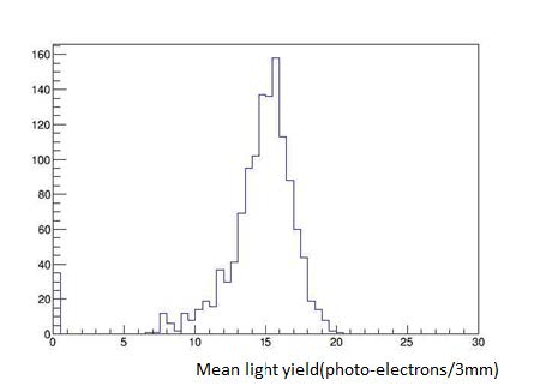
\includegraphics[width=0.5\linewidth]{fig/wmlight.pdf}
\end{center}
\caption{Light yield for muons produced by the interaction of neutrinos
  in the hall wall. Average light yields for each channel are plotted.
}
\label{fig:wmlight}
\end{figure}
A track search algorithm based on the cellular automaton has been developed using the software tools by the T2K INGRID. 
Examples of observed events are shown in Fig.~\ref{fig:onaxis_eventdisplay}
The tracking efficiency in 2-dimensional projected plane was evaluated by comparing the reconstructed track
in the WAGASCI module and the INGRID module and shown in Fig.\ref{fig:wmefficiency}.
Note that that the tracking efficiency for high angle ($>70\deg$) is not evaluated because of the acceptance
of the INGRID module, not because of the limitation of the WAGASCI module.
\begin{figure}[tbhp]
\begin{center}
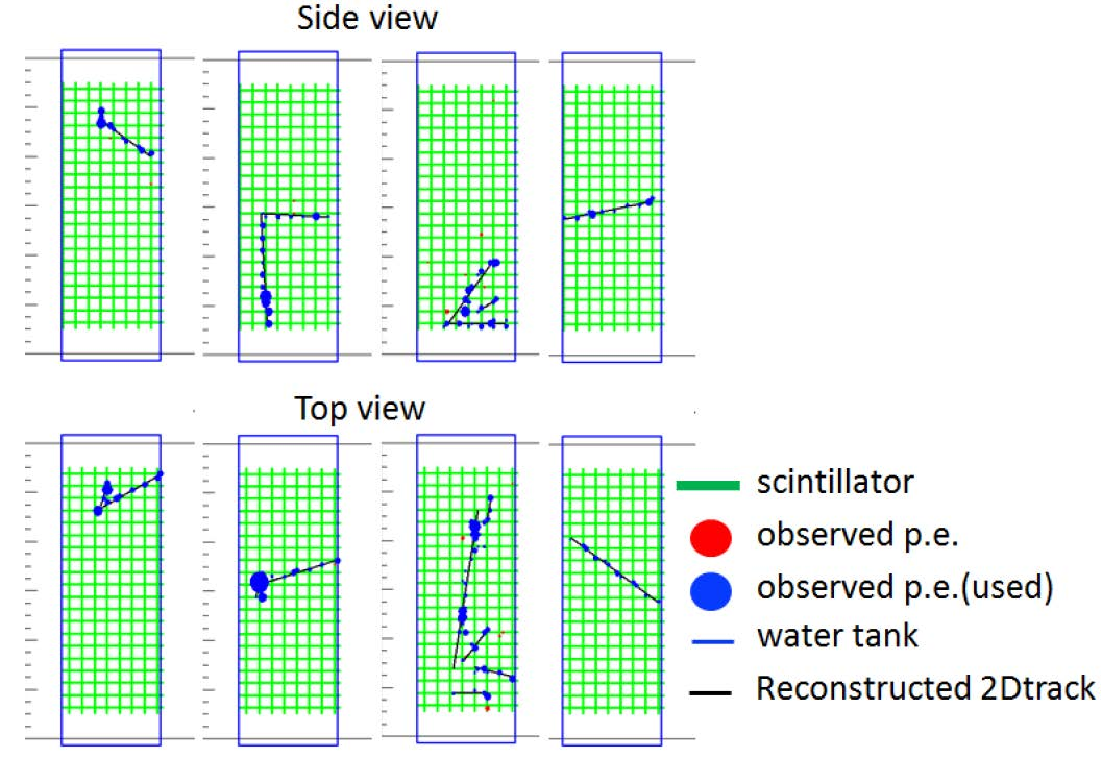
\includegraphics[width=\textwidth]{fig/wagascieventdisp.pdf}
%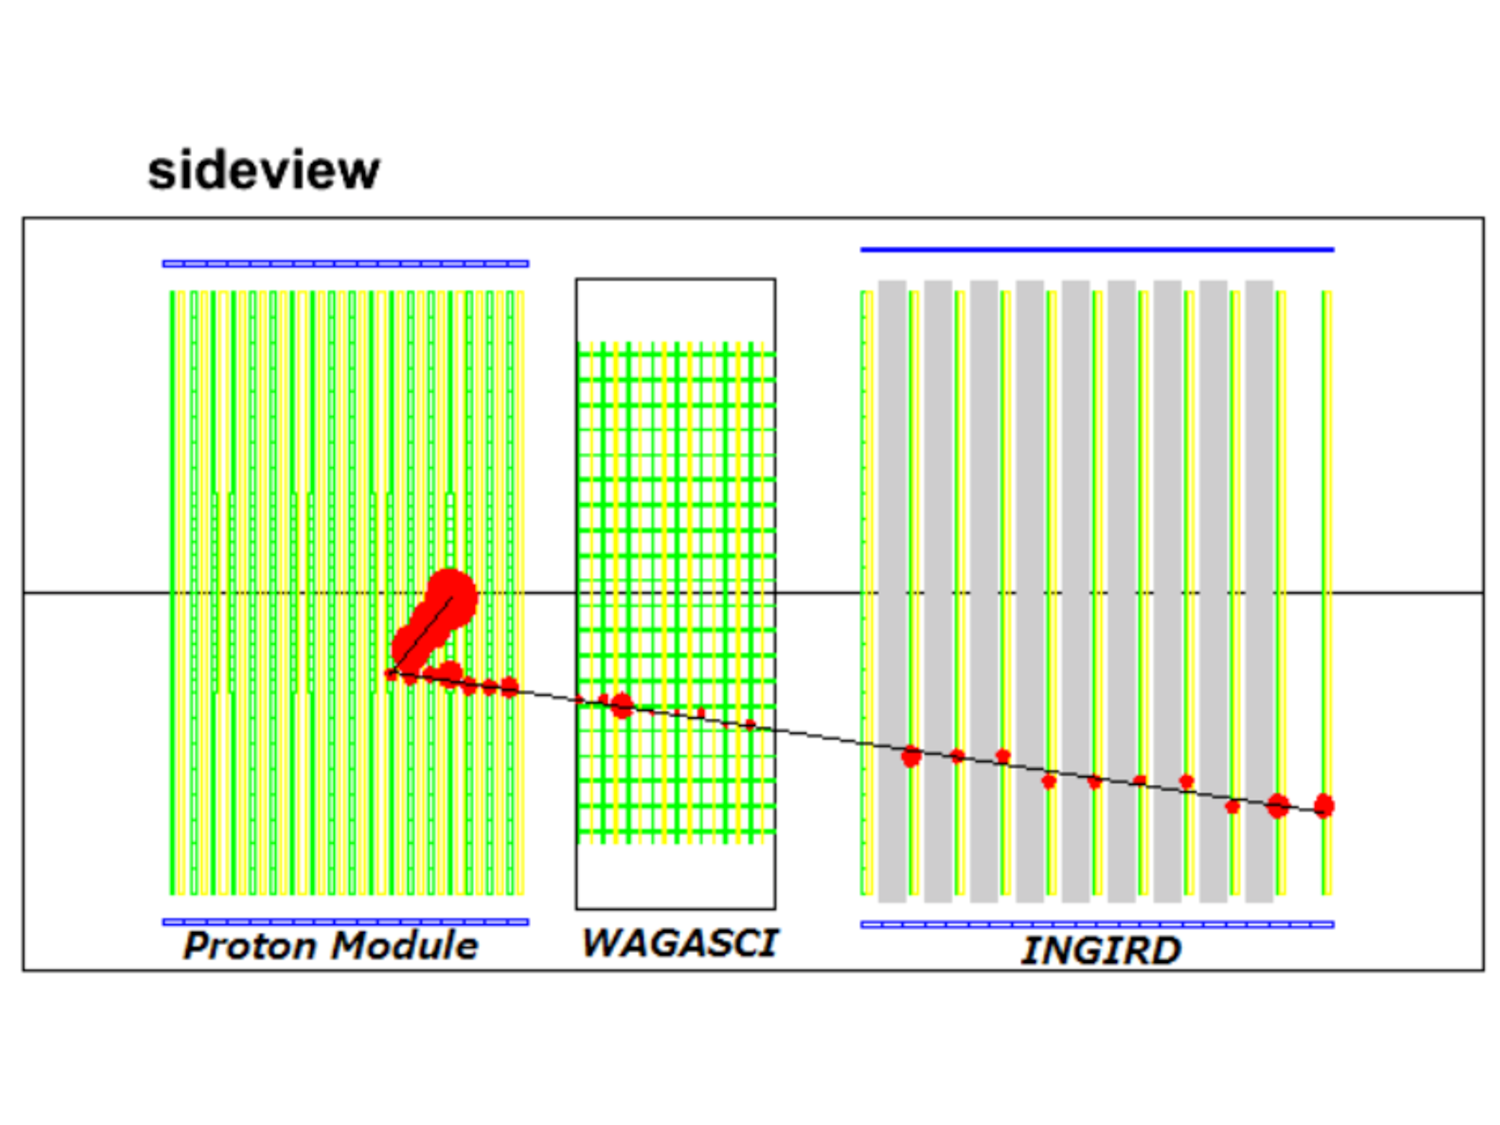
\includegraphics[width=0.8\linewidth]{fig/t59_event_display_oct_dec_2017.pdf}
% \includegraphics[width=0.8\linewidth]{fig/all_detector2.pdf}
\end{center}
\caption{
  Example event displays of the WAGASCI module at on-axis.
  The reconstructed tracks are overlaid.}
\label{fig:onaxis_eventdisplay}
%  t59_event_display_oct_dec_2017}
\end{figure}
%
\begin{figure}[tbhp]
  \begin{center}
   \begin{subfigure}{0.48\textwidth}
     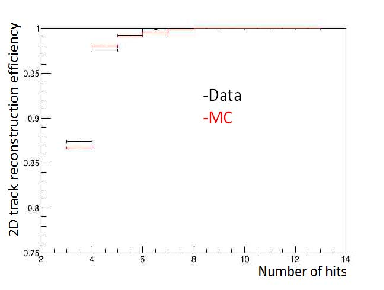
\includegraphics[width=\linewidth]{fig/wmeffvshit.pdf}
    \end{subfigure}
  \begin{subfigure}{0.48\textwidth}
      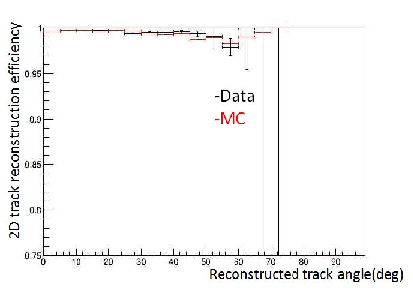
\includegraphics[width=\linewidth]{fig/wmeffvsangle.pdf}
    \end{subfigure}    
    \end{center}
  \caption{2D track reconstruction efficiency as a function of number of hits (left) and track angle (right).
  Here the track angle is the one reconstructed by the INGRID module.}
\label{fig:wmefficiency}
\end{figure}

In 2017 Autumn, the construction of the second WAGASCI module and the dedicated electronics board were completed.
The module and the electronics were install to the B2 floor together with the T2K proton module and the INGRID
module as shown in Fig.~\ref{fig:det_confg_oct_dec2017}.
The proton module is to be used as the entering muon veto and also for the comparison of interaction between CH and Water.
The INGRID module is for the temporary muon detector with limited acceptance for this period.
The detector was commissioned and is in operation to take data with the antineutrino beam during the T2K beam time from October.

 \begin{figure}[tbhp]
 \begin{center}
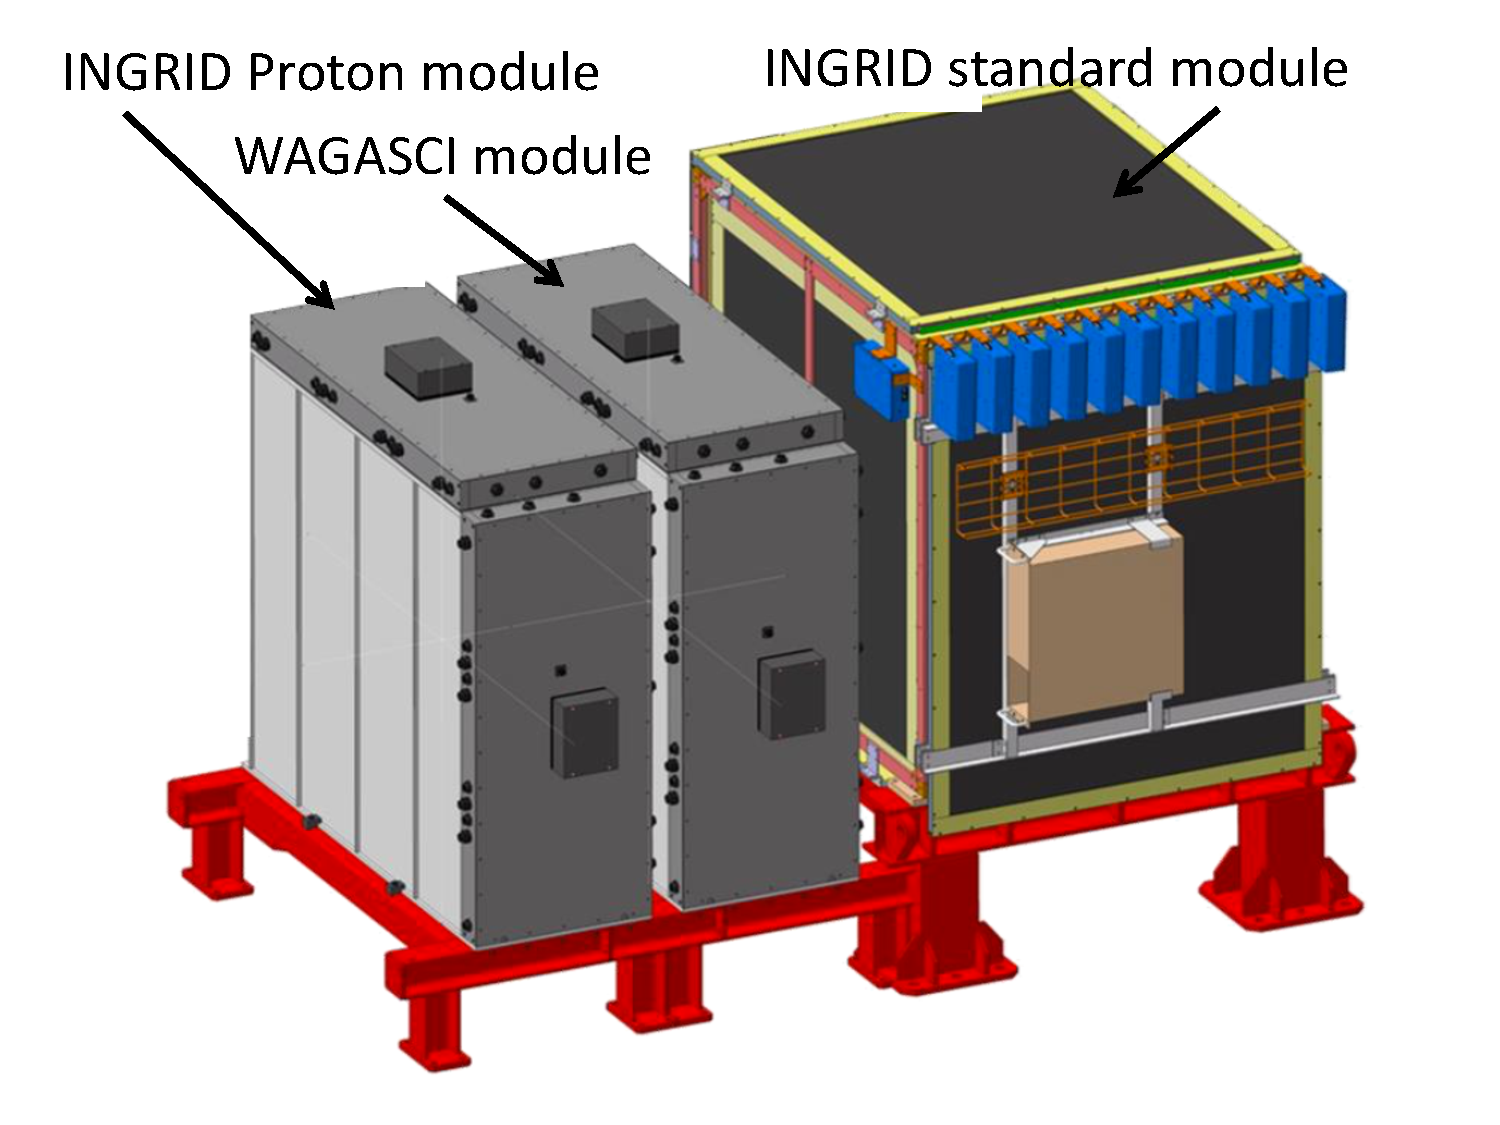
\includegraphics[width=0.5\linewidth]{fig/t59_det_config_oct_dec_2017.pdf}
 \end{center}
 \caption{
 J-PARC T59 detector configuration in October 2017.
 }
 \label{fig:det_confg_oct_dec2017}
 \end{figure}

The production of the components of the side muon range detectors has been completed and now the detectors
are being assembled at the Yokohama National University.
These detectors will be installed sometime from January to June, 2018 when T2K is not running.

The Baby MIND detector was transported from CERN to Japan in December, 2017.
It will be installed and commissioned in Jan.-Feb. 2018 and T59 will take the neutrino-induced muon data in April and May.

%Fist, the start time of neutrino beam measurement is changed from December 2015 to October 2017, and the requested neutrino beam is changed from $1\times10^{21}$ POT of $\nu$ beam to $0.8\times10^{21} $POT of anti-$\nu$ beam. 
% Second, the detector configuration is changed. In the original proposal, central neutrino detector are expected to be surrounded by newly developed muon-range detectors (MRDs), but we will use spare neutrino detectors of the T2K experiment instead of them during neutrino beam measurement from October to December 2017. Construction of the newly developed MRDs, Baby-MIND and Side-MRD, is in progress, and they will be installed to the both sides and the downstream of the central neutrino detector from January to March 2018. Then, we will resume neutrino beam measurements from March 2018 and will take the neutrino beam data until May 2018.


%\subsection{On-axis beam measurement with Prototype detector}
%Add INGRID water module measurement here.

%\subsection{Plans from October 2017 to May 2018}
%J-PARC MR will extract its proton beam to T2K neutrino beam-line from October to December 2017, and, from March to May 2018. 
%T2K experiment will produce anti-neutrino beam and will accumulate $\sim8\times10^{20}$ POT data during the above period.


% J-PARC T59 will perform neutrino beam measurements on the B2 floor of the T2K near neutrino detector hall during the above period to test basic performances of the WAGASCI detector and new electronics. During the beam measurements from October to December 2017, one WAGASCI module will be placed between spare neutrino detectors of the T2K experiment, INGRID Proton module and INGRID standard module. 
 % as shown in Fig. \ref{fig:det_config_oct_dec2017}.
% Detector location on the B2 floor of T2K near detector hall is shown in Fig. \ref{fig:det_loc_oct_dec2017}. 
%Here, the INGRID Proton module is used as a charged particle VETO detector and, the INGRID standard module is used as a downstream muon detector. 
%We had submitted a proposal to use these spare neutrino detectors for the T59 neutrino beam measurements to the T2K collaboration, and we got an approval from T2K. 


 
% \begin{figure}[tbh]
% \begin{center}
% 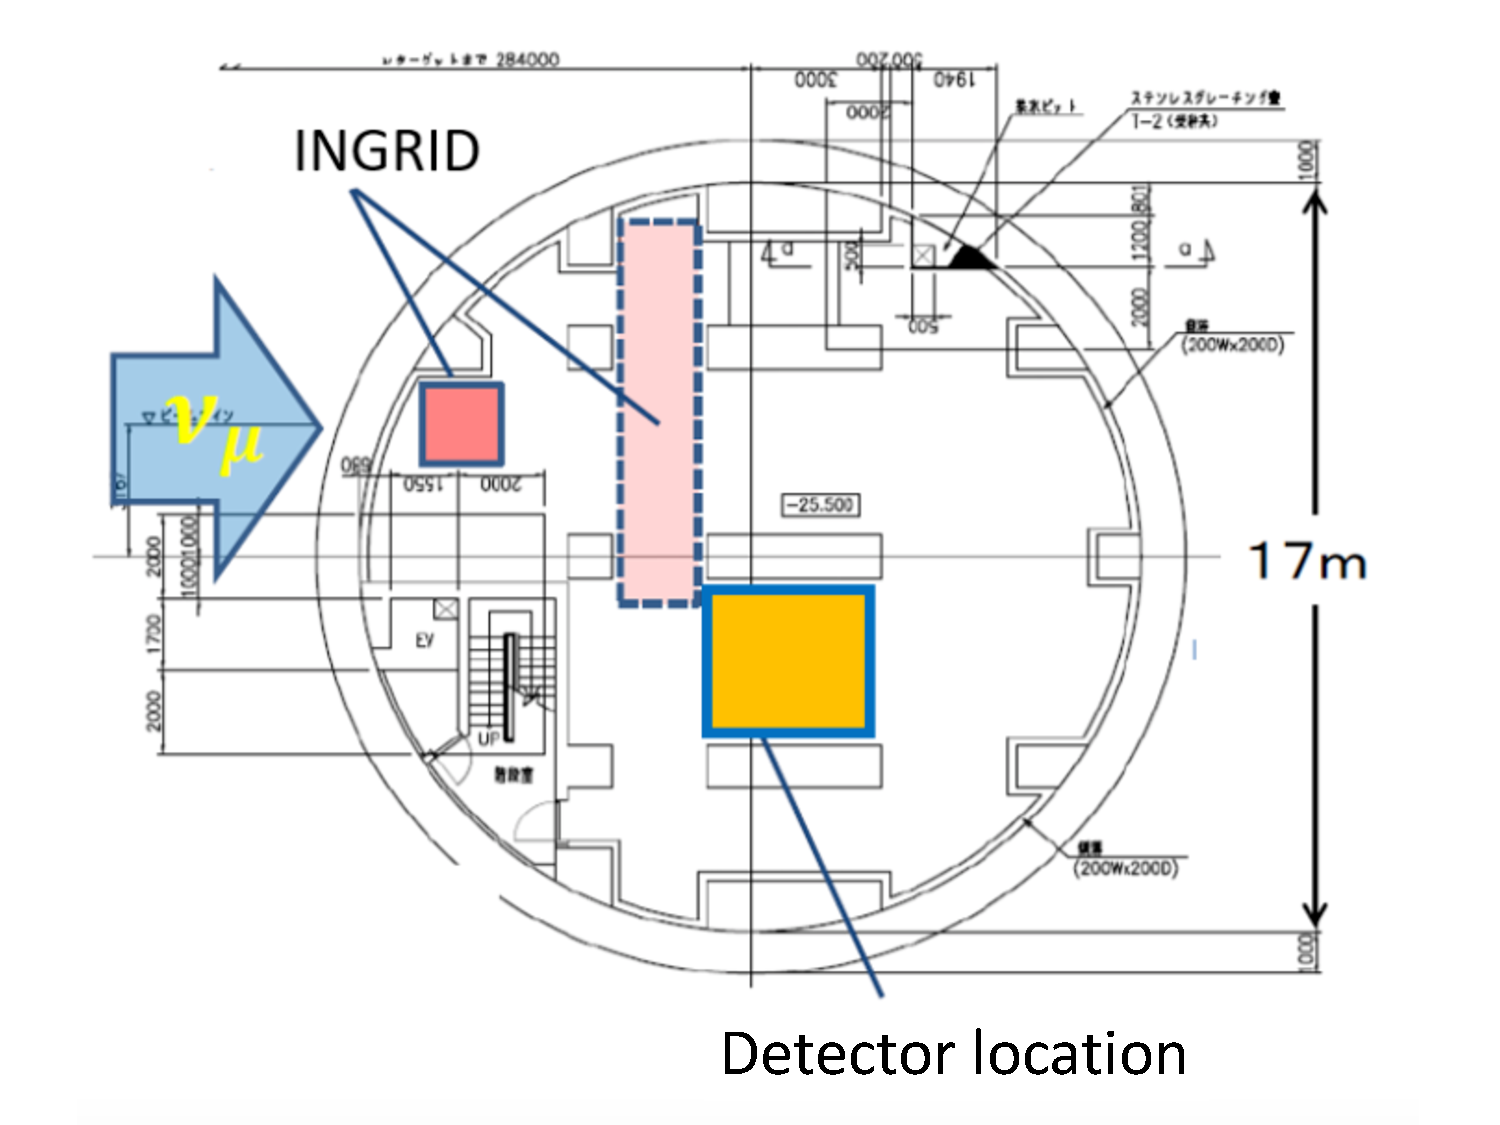
\includegraphics[width=0.8\linewidth]{fig/t59_det_location_oct_dec_2017.pdf}
% \end{center}
% \caption{
% J-PARC T59 detector location from Oct. to Dec. 2017
% }
% \label{fig:det_loc_oct_dec2017}
% \end{figure}


%During the beam measurements from March to May 2018, Baby-MIND and two side muon-range detector (Side-MRD) modules will be installed on the downstream and the both sides of the WAGASCI detector, as shown in Fig. \ref{fig:det_config_mar_may2018}, to increase angular acceptance for secondary charged particles from neutrino interactions.
 
%\begin{figure}[tbh]
%\begin{center}
%
\includegraphics[width=0.8\linewidth]{fig/tmp.pdf}
% \includegraphics[width=0.8\linewidth]{fig/all_detector2.pdf}
%\end{center}
%\caption{
%J-PARC T59 detector configuration with Baby-MIND and two Side-MRD modules from Mar. to May 2018.
%(Need to prepare the figure.)}
%\label{fig:det_config_mar_may2018}
%\end{figure}


%Expected number of neutrino events in the WAGASCI detector during the above beam period is evaluated with Monte Carlo simulations. 
%Neutrino beam flux at the detector location is simulated by T2K neutrino flux generator, JNUBEAM, neutrino interactions with target materials are simulated by a neutrino interaction simulator, NEUT, detector responses are simulated using GEANT4-based simulation. 
%The neutrino flux at the detector location, 1.5 degrees away from the J-PARC neutrino beam axis, is shown in Figure \ref{fig:b2flux}, and its mean neutrino energy is around 0.68 GeV.


%To perform the detector performance test, the following event selections are applied to the data. 
%First, track reconstructions are performed in the WAGASCI detector, and the reconstructed vertex is required to be inside a defined fiducial volume, $80 \times80 \times 32$ cm$^{3}$ region at the center of the detector, to reduce contamination from external backgrounds. 
%Second, at least one charged particle is required to reach to INGRID standard module or Side-MRD modules, and it makes more than two hits in these sub-detectors. 
%With the event selection, expected numbers of the neutrino-candidate events during the beam period are summarized in Table 1. 
%Using the data, we will test the detector performance with $\sim3$\% statistical uncertainties.









\section{MC studies}
\label{sec:mc_study}
\subsection{Simulation setup}
\label{sec:mc_setup}
The expected number of neutrino events in the water-in Wagasci detector
is predicted by Monte Carlo simulations.
Neutrino beam flux at the detector location is simulated by T2K neutrino flux generator, JNUBEAM. Neutrino interactions with target materials are simulated by a neutrino interaction simulator, NEUT. Detector responses are simulated using GEANT4-based simulation.


The detector geometry in the simulation so far is different from the actual setup as shown in Figure \ref{fig:wagasci_mc_geometry}.
The active neutrino target region consists of four WAGASCI modules.
The size of the WAGASCI module is same as the actual one: 1000 mm $\times$ 1000 mm in the x and y directions and 500 mm along the beam direction (z-direction).
%An event display of a MC event in the WAGASCI detectors is shown in Figure \ref{fig:wagasci_event_display}.
Two Side-MRD modules are installed either side of the Wagasci modules.
Each Side-MRD module consists of ten iron plates whose dimension is 30 mm (thickness) $\times$ 2000 mm (height) $\times$ 3200 mm (width). 
The distance between the Side-MRD modules and WAGASCI modules is 800 mm.
The downstream-MRD is equivalent to the Baby-MIND, but without the magnetic field.
It consists of thirty iron plates whose dimension is  30 mm (thickness) $\times$ 2000 mm (height) $\times$ 4000 mm (width).
The distance between the downstream-MRD modules and WAGASCI modules is 800 mm.
Update of the study with the actual geometry is now underway.

\begin{figure}[tbhp]
\begin{center}
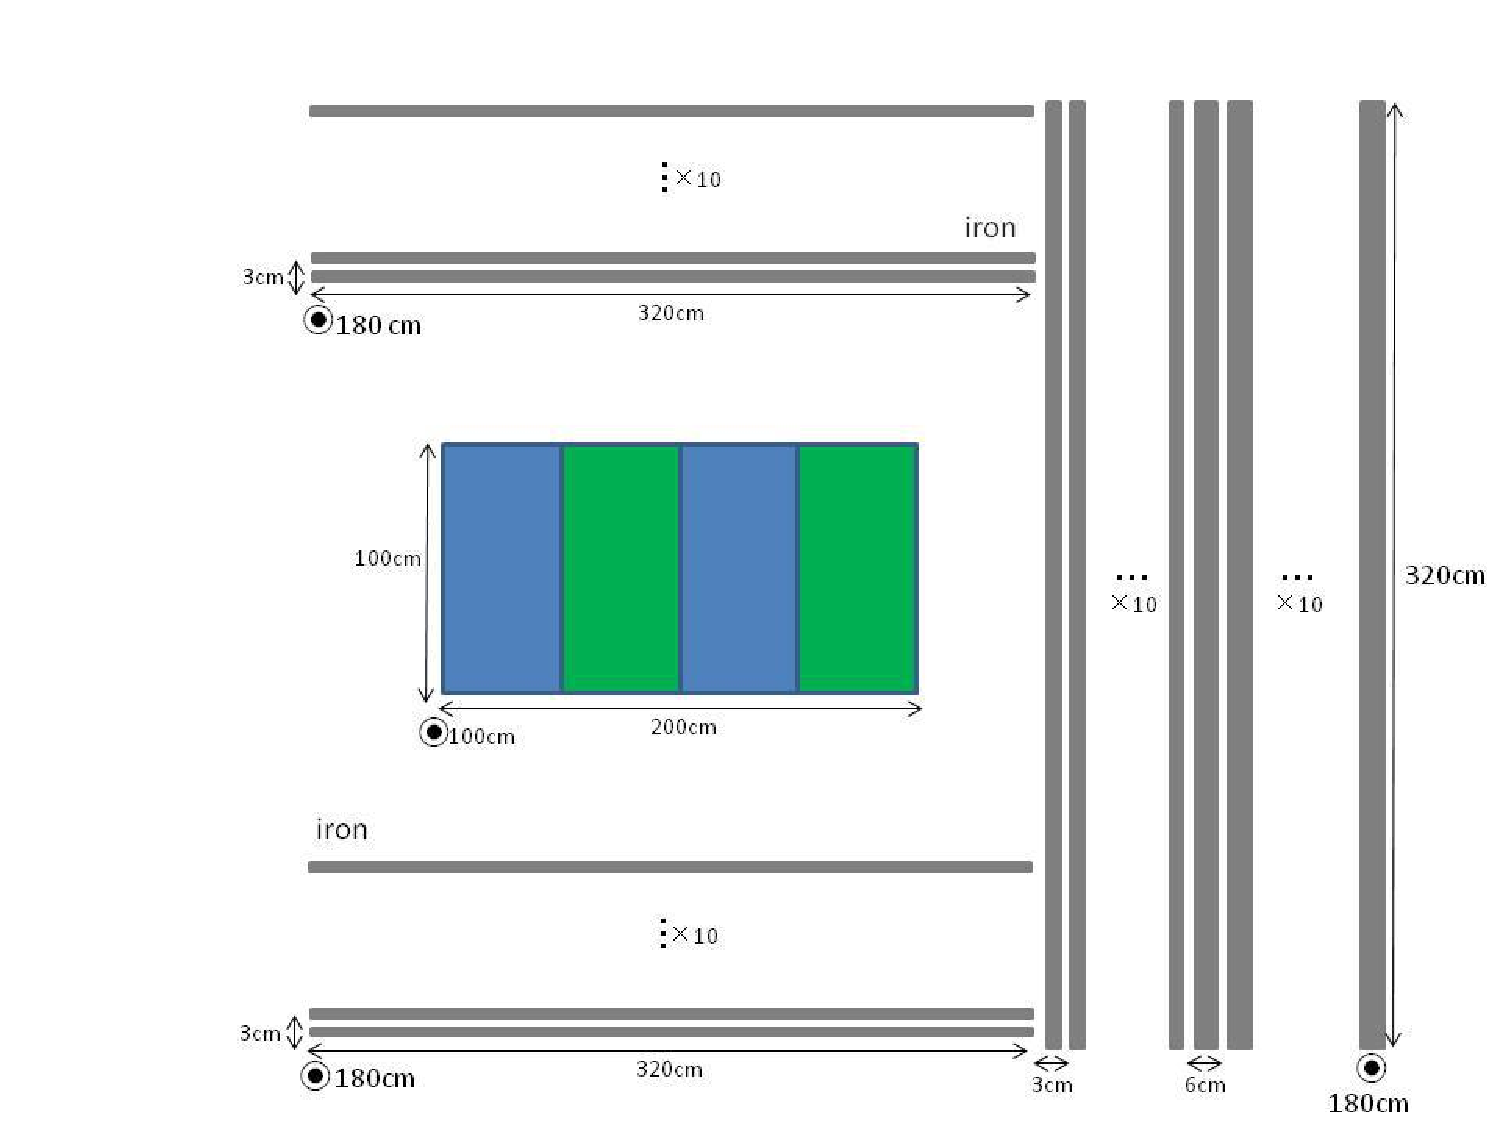
\includegraphics[width=0.8\linewidth]{fig/wagasci_mc_geometry.pdf}
% \includegraphics[width=0.8\linewidth]{fig/all_detector2.pdf}
\end{center}
\caption{
Geometry of the detectors in the Monte Carlo simulation.}
\label{fig:wagasci_mc_geometry}
\end{figure}

%\begin{figure}[tbh]
%\begin{center}
%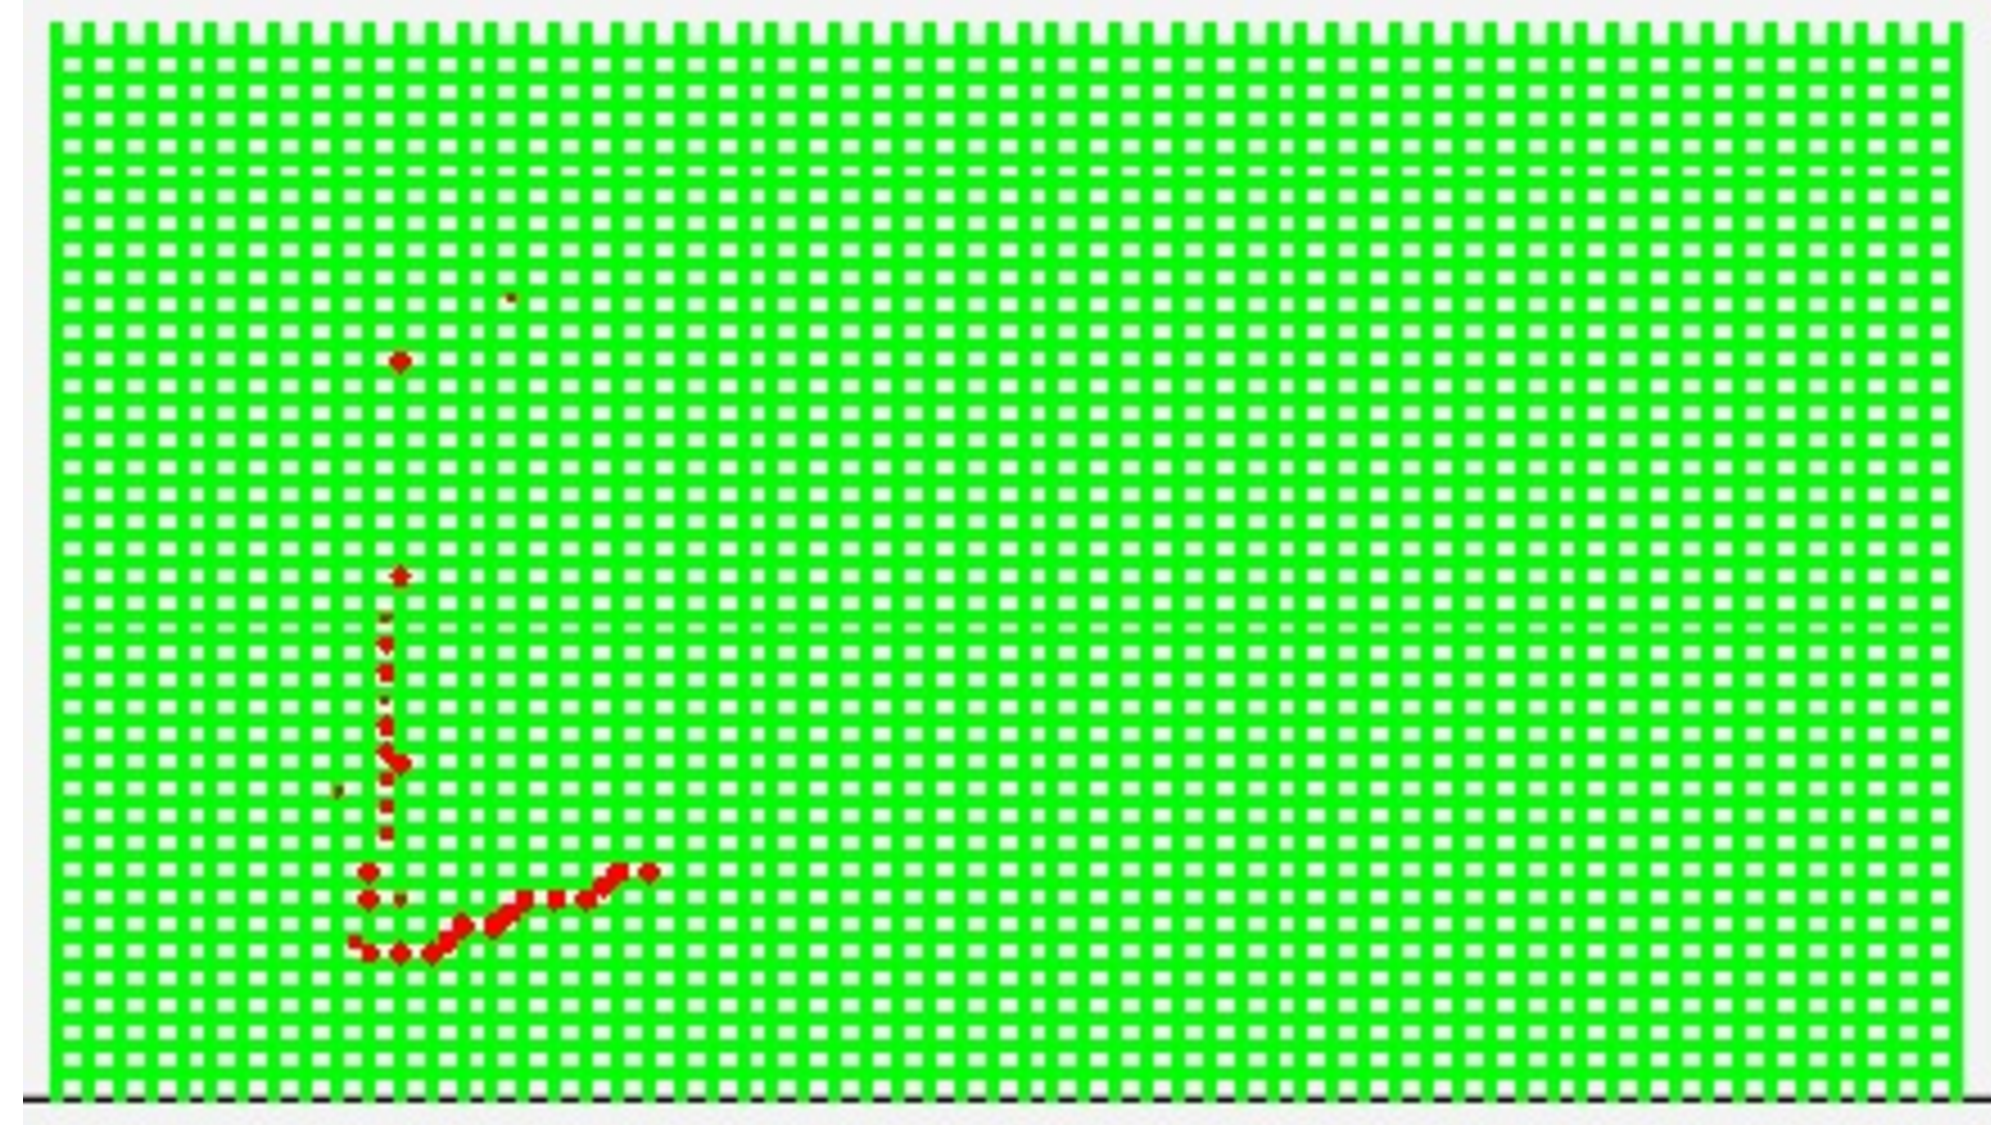
\includegraphics[width=0.8\linewidth]{fig/wagasci_event_display.pdf}
%% \includegraphics[width=0.8\linewidth]{fig/all_detector2.pdf}
%\end{center}
%\caption{
%An event display of MC event in WAGASCI detectors. Green lines are scintillators and red circles are the hit channels.}
%\label{fig:wagasci_mc_geometry}
%\end{figure}

% In order to estimate backgrounds from neutrino interactions in the wall and floor of the experimental hall, the geometry of the experimental hall is implemented in the GEANT4-based detector simulation.

To simulate the signal, the energy deposit inside the scintillator is converted into the number of photons. 
The effects of collection and attenuation of the light in the scintillator and the WLS fiber are simulated, and the MPPC response is also taken into account. 
The light yield is smeared according to statistical fluctuations and electrical noise.


\subsection{Charged-current event selection}

Tracks are reconstructed in two-dimensional planes in each sub-detector.
Then, track matching among the sub-detectors and three-dimensional track reconstruction are performed.
These analysis tools have been developed from the software tools by the T2K INGRID and in mature stage already.

The events are selected as follows.
The starting point of the track is required to be 50~mm away from the edge of the WAGASCI module. This is to remove the background from the outside.
% as shown in Fig. \ref{fig:fv_cut}.
% \begin{figure}[tbh]
% \begin{center}
%   \begin{subfigure}{0.48\textwidth}
%     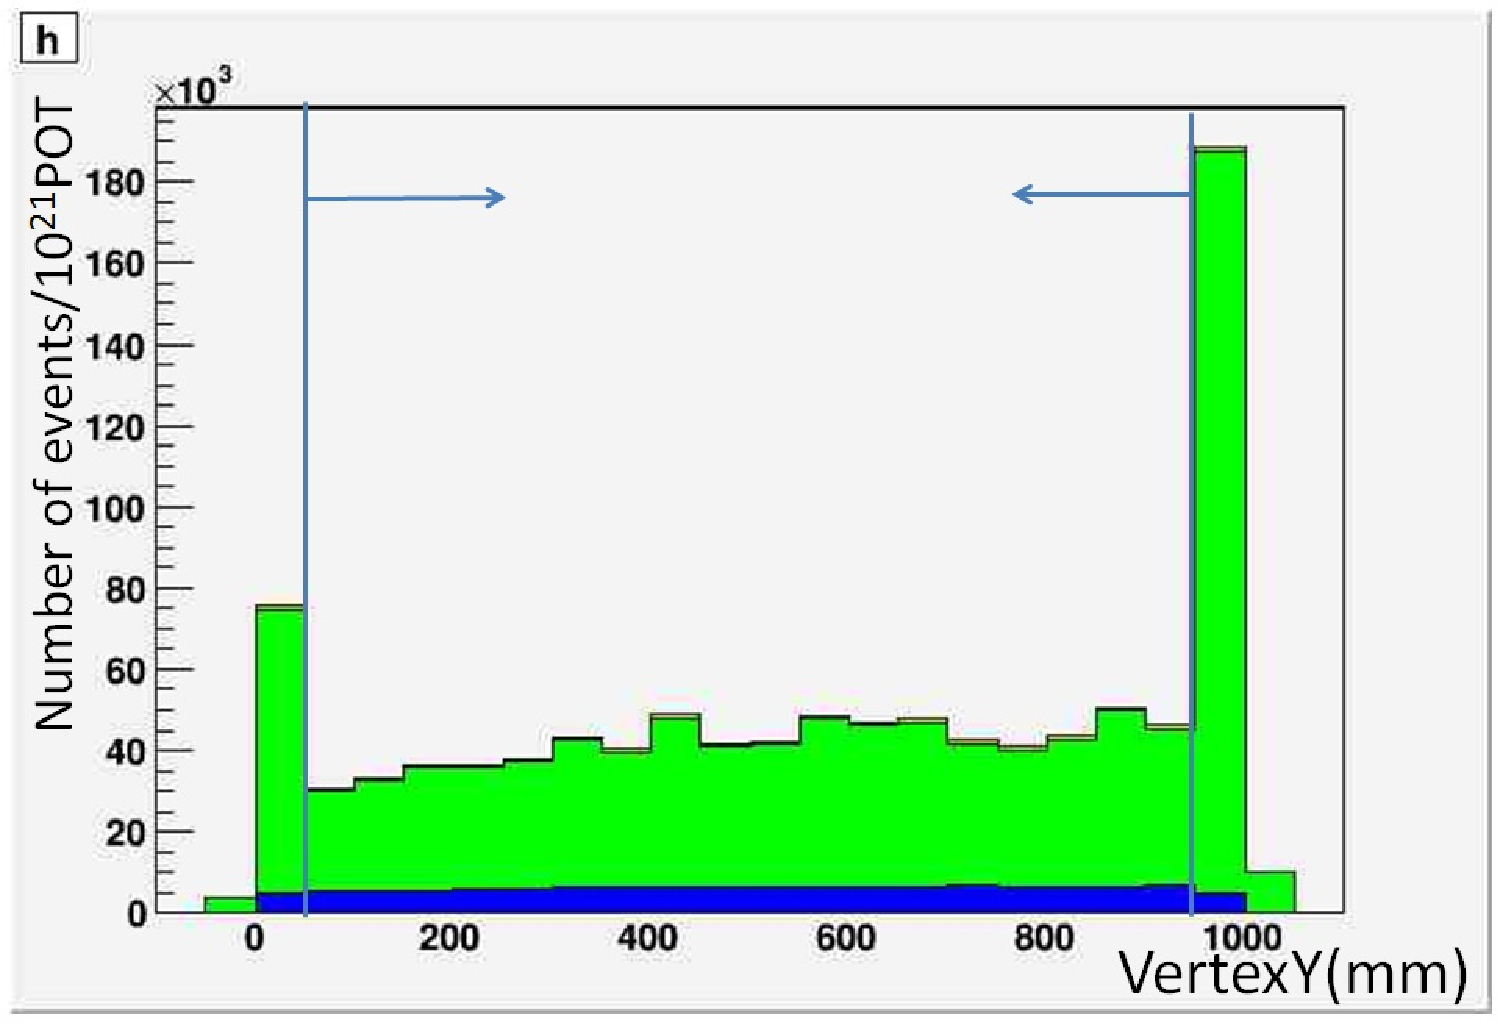
\includegraphics[width=\linewidth]{fig/fv_cut_y.pdf}
%    \end{subfigure}
%  \begin{subfigure}{0.48\textwidth}
%      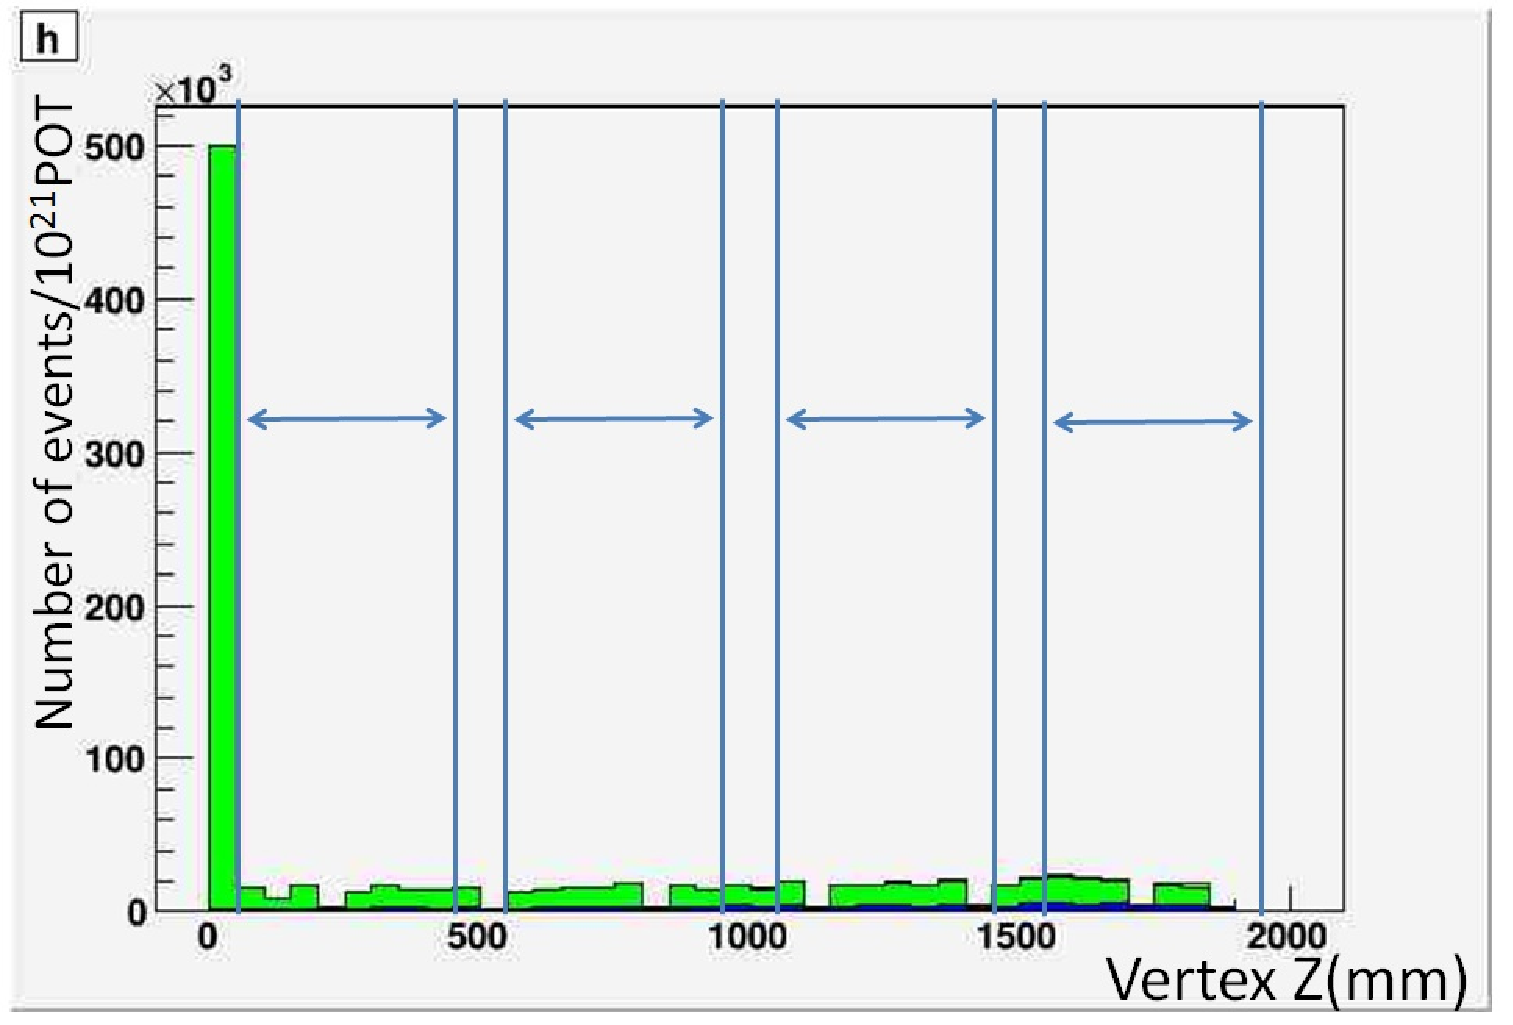
\includegraphics[width=\linewidth]{fig/fv_cut_z.pdf}
%    \end{subfigure}    
%    \end{center}
%  \caption{Event selection with the vertex of the track.
% Blue hist. are events from the WAGASCI modules, green hist. are events from the experimental hall, % and yellow hist. are events from the Side-MRD modules and the downstream-MRD.
% }
% \label{fig:fv_cut}
% \end{figure}
The longest track has to penetrate more than one (five) iron plates in Side-MRD modules (Baby-MIND).
This cut select a muon track and rejects backgrounds from NC and neutral particles.
%as shown in Figure \ref{fig:penetrated_iron_plates_cut}.
Then, in order to determine the muon momentum, it is required that the longest track stops in MRDs (Side-MRD modules and Baby-MIND) or penetrate all iron plates.
% \begin{figure}[tbh]
%  \begin{center}
%   \begin{subfigure}{0.48\textwidth}
%      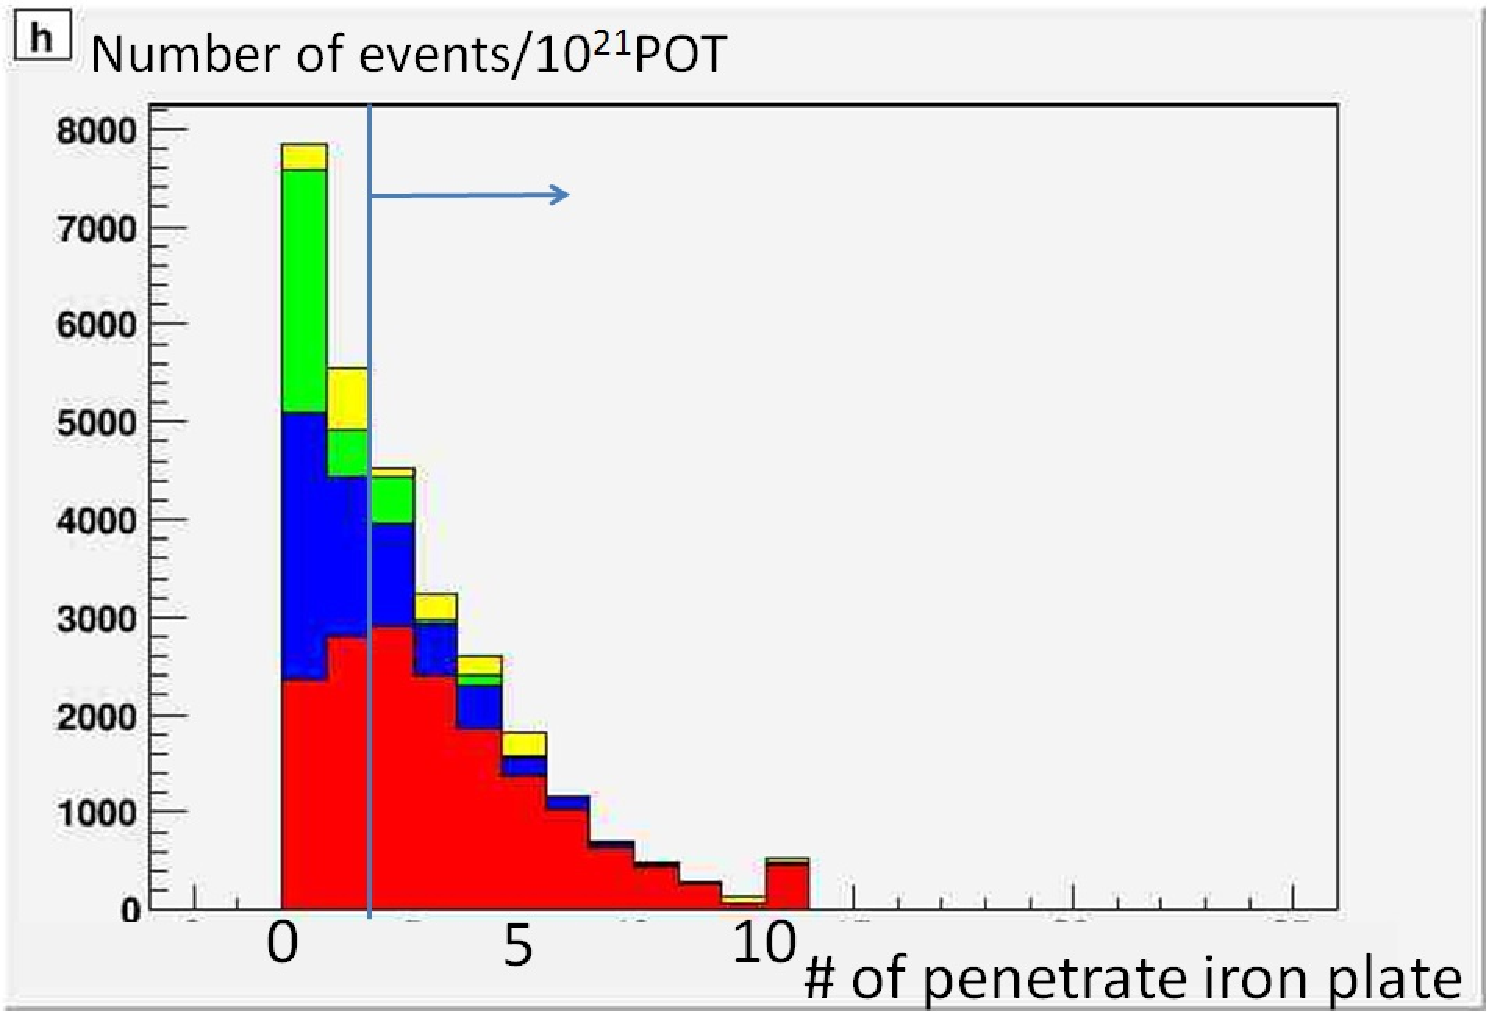
\includegraphics[width=\linewidth]{fig/penetrated_iron_plates_cut_sidemrd.pdf}
%     \end{subfigure}
%   \begin{subfigure}{0.48\textwidth}
%     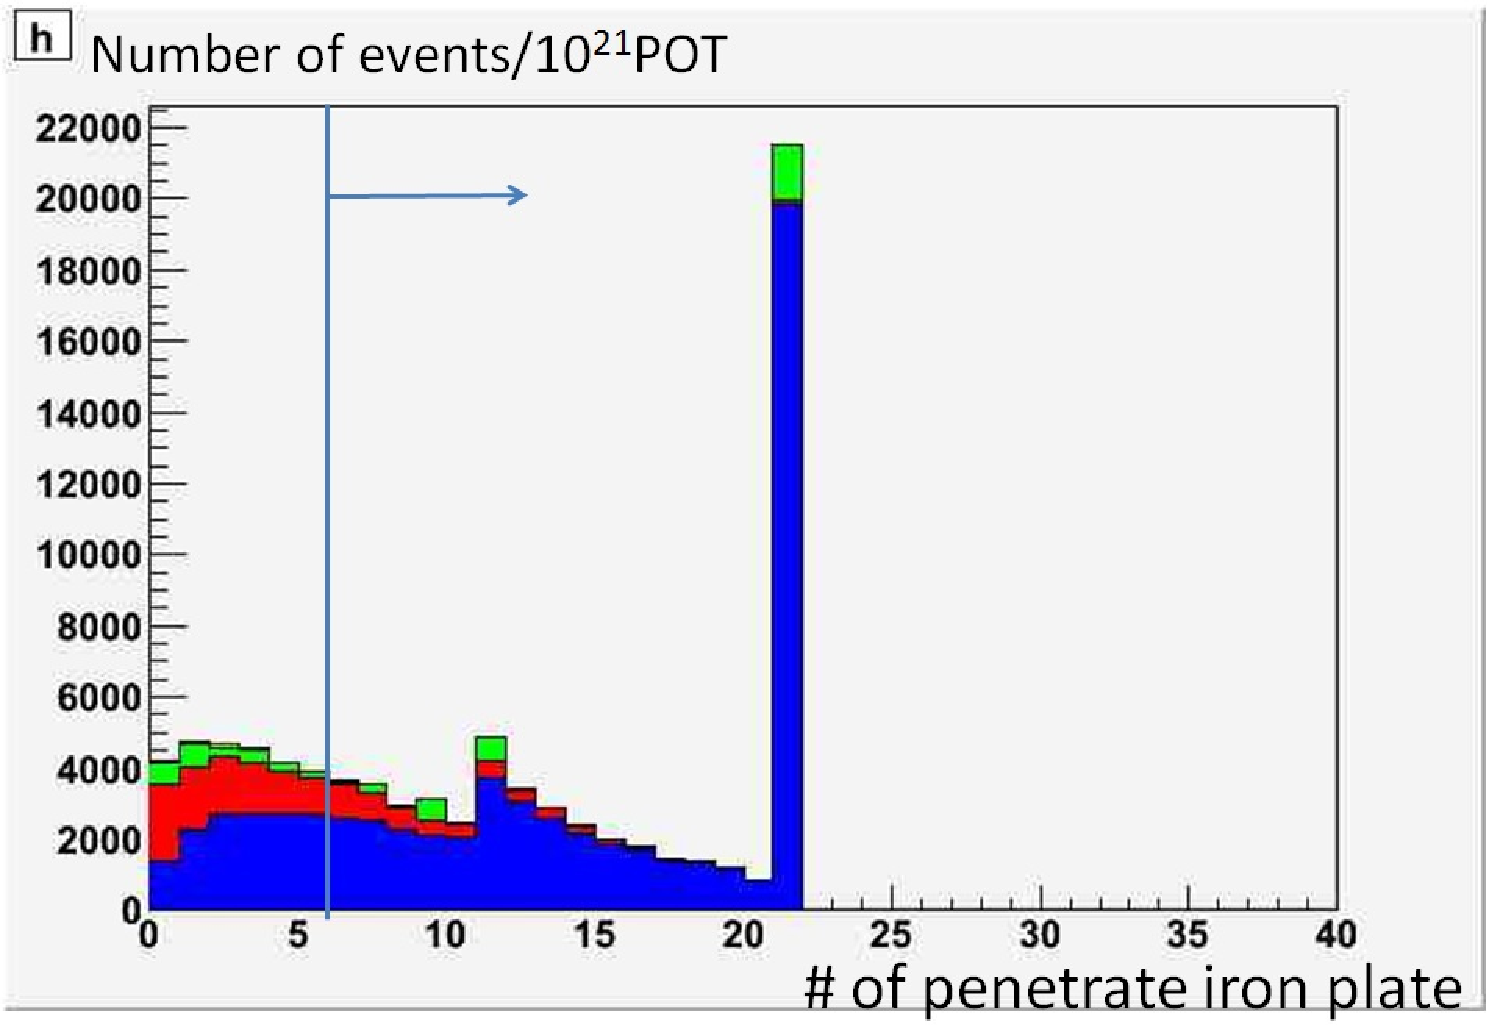
\includegraphics[width=\linewidth]{fig/penetrated_iron_plates_cut_babymind.pdf}
%     \end{subfigure}    
%     \end{center}
%   \caption{
% Event selection with the number of the penetrated iron plates in the side-MRD modules (left) and the Baby-MIIND (right).
% Blue and red hist. are events from the WAGASCI modules, green hist. are events from the experimental hall, and yellow hist. are events from the Side-MRD modules and the Baby-MIND.
% }
% \label{fig:penetrated_iron_plates_cut}
% \end{figure}

% \subsection{Selected events}


Table~\ref{tab:expected_num_events}  shows numbers of the selected events in one water-in WAGASCI module after the event selection.
We expect 4,239 (1,666) events from charged-current interaction on $\mathrm{H_2O}$ with $5 \times 10^{20}$  POT in (anti)neutrino-mode with one water-in WAGASCI module.
The purity, when interactions on CH is counted as background, is 78\% for the neutrino-mode.
There is a significant contamination from the wrong-sign (neutrino) interaction for antineutrino-mode, however, we expect that
it will be removed with efficiency higher than 90\% by Baby MIND.
%\begin{table}[htb]
%  \begin{center}
%    \caption{Expected number of the neutrino-candidate events in one water-in WAGASCI module with 1$\times 10^{21}$ POT in neutrino-mode.}
%    \begin{tabular}{c|ccc|c} \hline
%Cut   & CC & NC & Scinti Bkg. & Total \\ \hline
%Reconstructed & 18093.2 & 699.7 & 4698.3 & 23491.2 \\
%FV & 15150.8 & 588.4 & 3934.8 & 19673.9 \\
%Pene. iron & 11264.3 & 237.3 & 2875.4 & 14377.0 \\
%Stop/Penetrate MRDs & 8478.2 & 214.0 & 2173.1 & 10865.2 \\ \hline
%after all cuts & 78.0 \% & 2.0 \% & 20.0 \% & 100 \% \\
%\hline
%    \end{tabular}
%    \label{tab:expected_num_events_neutrino_beam}
%  \end{center}
%\end{table}
%\begin{table}[htb]
%  \begin{center}
%    \caption{Expected number of the antineutrino-candidate events in one water-in WAGASCI module with 1$\times 10^{21}$ POT in antineutrino-mode.}
%    \begin{tabular}{c|cccc|c} \hline
% Cut   & CC & NC & Scinti Bkg. & Wrong sign bkg & Total \\ \hline
%Reconstructed & 6499.7 & 107.3 & 2234.4 & 2330.8 & 11172.1 \\ 
%FV & 5457.9 & 89.3 & 1873.5 & 1946.6 & 9367.1 \\ 
%Pene. iron & 4172.3 & 30.8 & 1440.9 & 1560.6 & 7204.6 \\ 
%Stop/Penetrate MRDs & 3331.5 & 28.5 & 1120.3 & 1121.2 & 5601.5 \\ \hline
%after all cuts & 59.5 \% & 0.5 \% & 20.0 \% &  20.0 \% & 100 \% \\
%\hline
%    \end{tabular}
%    \label{tab:expected_num_events_antineutrino_beam}
%  \end{center}
%\end{table}
\begin{table}[htbp]
  \begin{center}
    \caption{Expected number of the selected neutrino-candidate events in one water-in WAGASCI module with $5\times 10^{20}$ POT in each of neutrino-mode and antineutrino-mode.
      Note that the wrong sign component will be reduced by one order by applying the charge selection by Baby MIND.}
    \begin{tabular}{ccccc} \hline
   & CC on $\mathrm{H_2O}$ & NC on $\mathrm{H_2O}$ & Interaction on CH  & wrong sign interaction\\ \hline
   $\nu$-mode & 4239 & 107 & 1087 & (negligible) \\ \hline
   anti-$\nu$-mode & 1666 & 14 & 560 & (561) \\
\hline
    \end{tabular}
    \label{tab:expected_num_events}
  \end{center}
\end{table}


Table \ref{tab:expected_num_cc_events} and \ref{tab:expected_num_ccfsi_events} summarize
contributions classified by the interaction types and final state topologies for the selected charged current-interaction events, respectively.
%
\begin{table}[htbp]
  \begin{center}
    \caption{Interaction types for the selected charged-current events.}
    \begin{tabular}{c|cccc} \hline
& CCQE & 2p2h & CC resonant $\pi$  & CC-DIS \\ \hline
$\nu$-mode & 48.4 \% & 9.7 \% & 27.1 \% & 14.7 \% \\
anti-$\nu$-mode &  57.1 \% & 8.2 \% & 17.3 \% & 17.3 \% \\
\hline
    \end{tabular}
    \label{tab:expected_num_cc_events}
  \end{center}
\end{table}
%
\begin{table}[htbp]
  \begin{center}
    \caption{Final state topologies for the selected charged-current events.}
    \begin{tabular}{c|cccc} \hline
& CC0$\pi$ & CC1$\pi$ & CC2$\pi$ & CCn$\pi$ \\ \hline
      $\nu$-mode & 67.4 \% & 20.9 \% & 3.0 \% & 8.7 \% \\ \hline
      anti-$\nu$-mode & 79.5 \% & 16.3 \% & 1.2 \% & 3.0 \% \\\hline
    \end{tabular}
    \label{tab:expected_num_ccfsi_events}
  \end{center}
\end{table}

Figure \ref{fig:angle_allcut} shows the reconstructed angles of the longest tracks in the selected events in the neutrino-mode and the anti-neutrino mode.
Figure \ref{fig:endpoint_longest_track} shows the iron plane numbers in Side-MRD and Baby-MIND corresponding to the end points of the longest tracks in the selected events in the neutrino-mode and the anti-neutrino mode.
%
\begin{figure}[tbh]
 \begin{center}
  \begin{subfigure}{0.48\textwidth}
     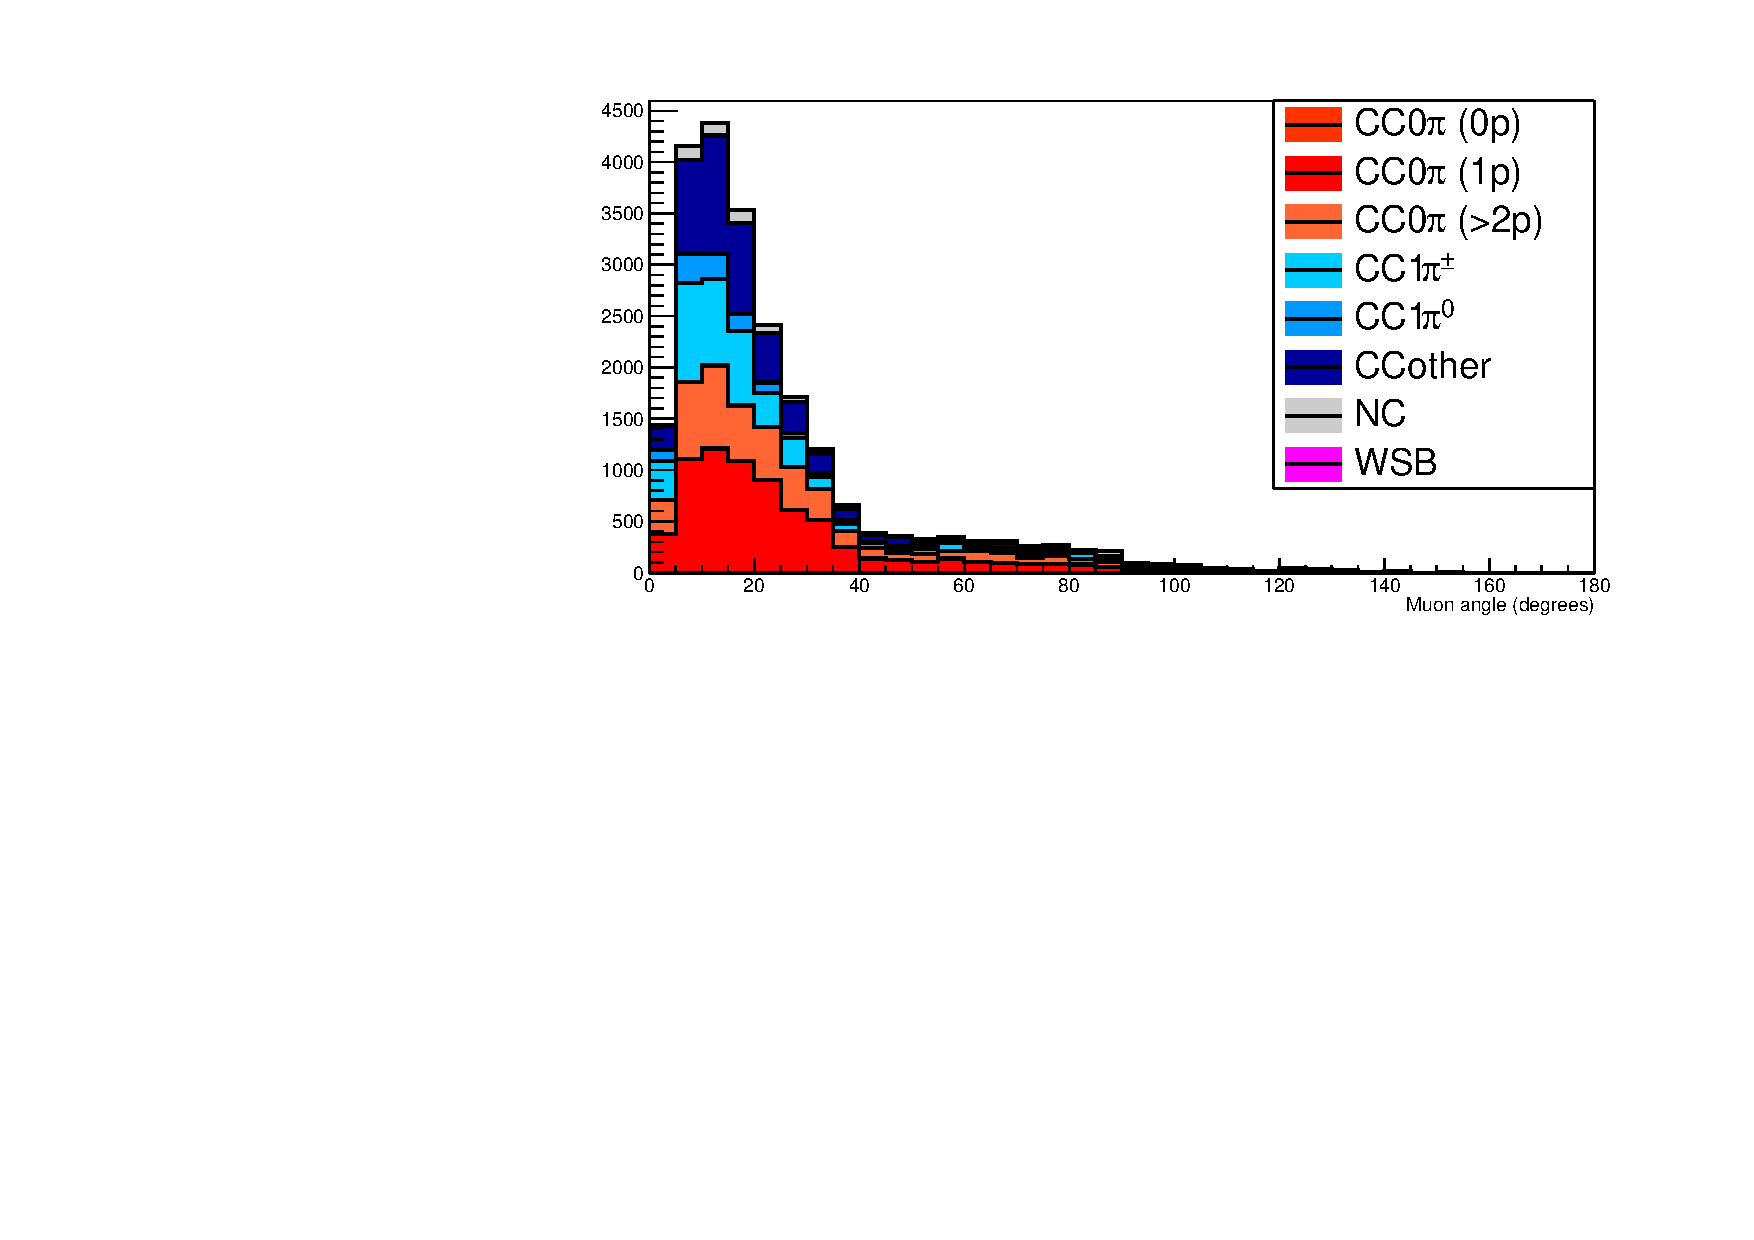
\includegraphics[width=0.55\linewidth, angle=270]{fig/FHCMuonAngle_StoppedOrThroughGoing.pdf}
%     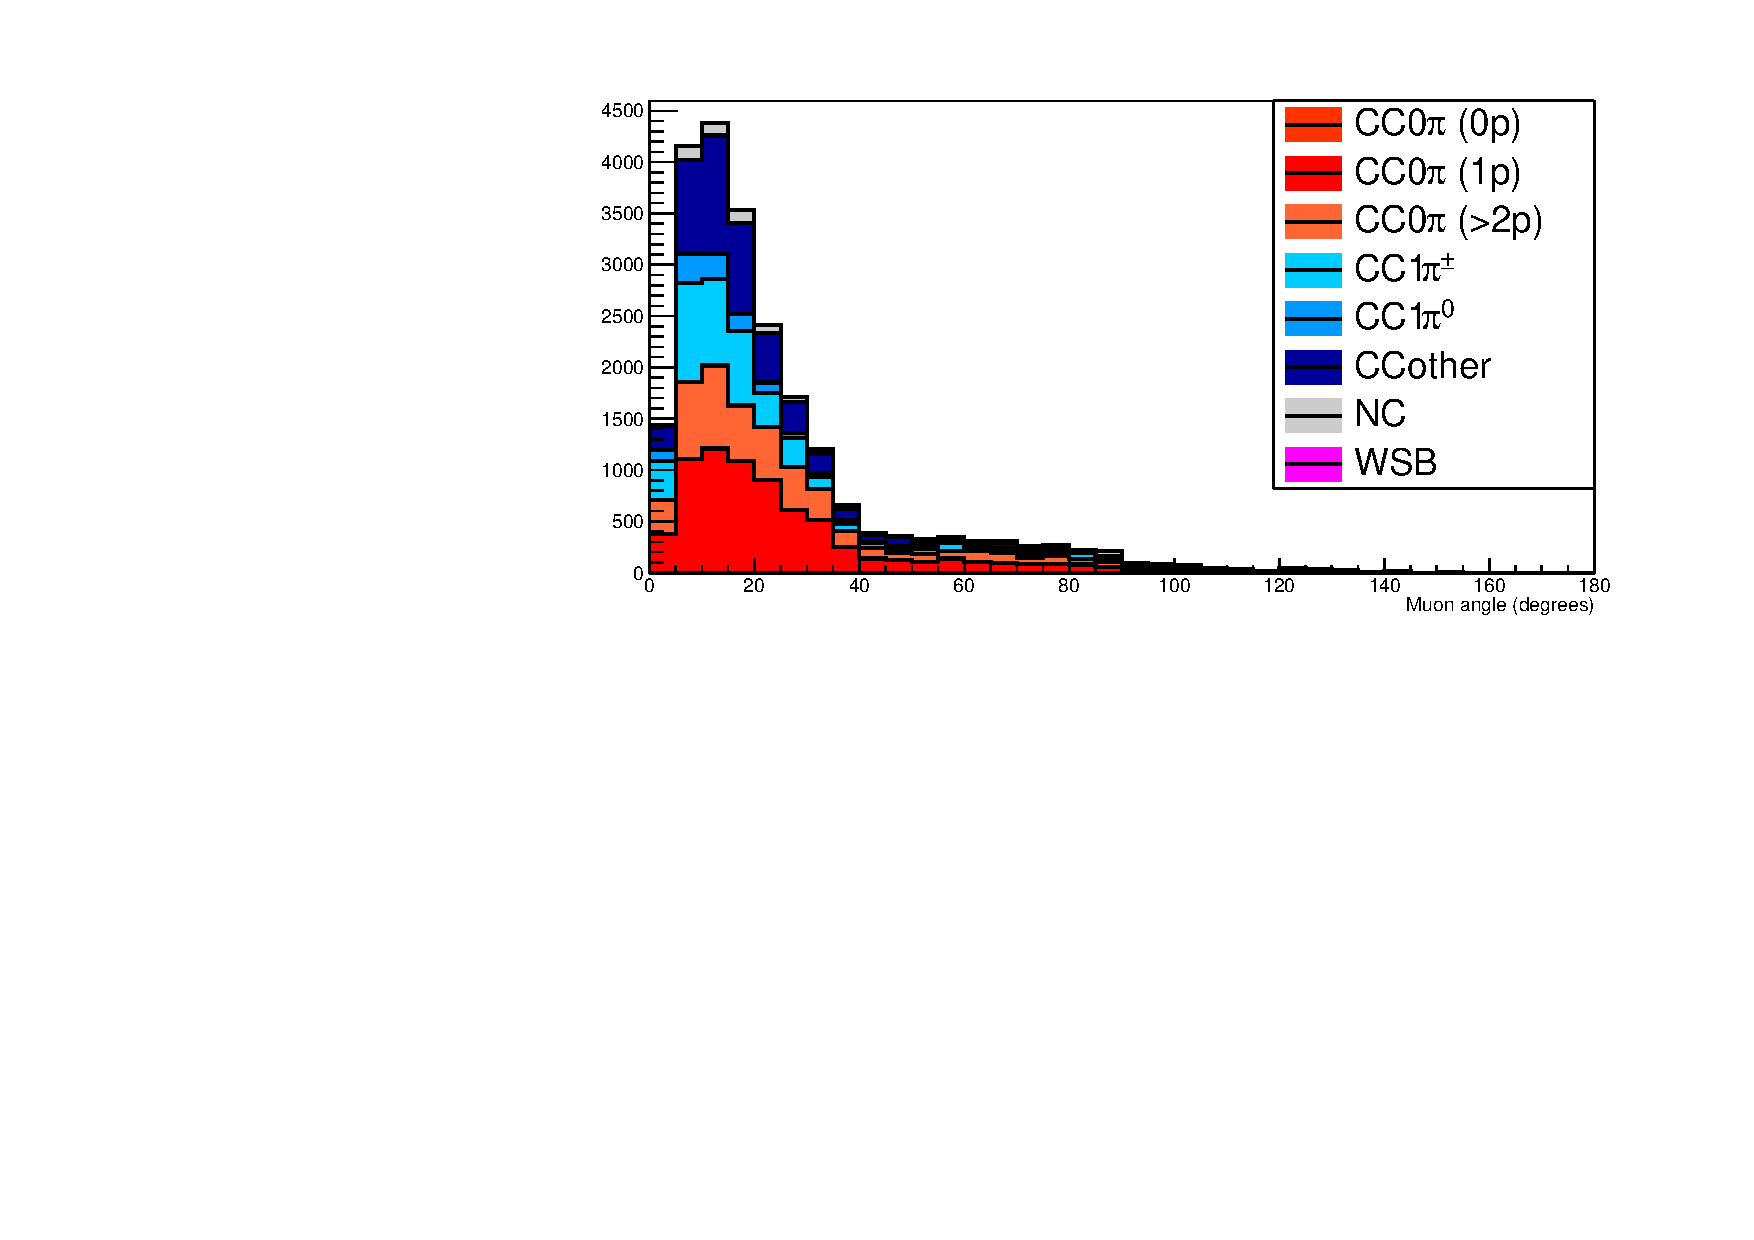
\includegraphics[width=\textwidth]{fig/FHCMuonAngle_StoppedOrThroughGoing.pdf}
    \end{subfigure}
  \begin{subfigure}{0.48\textwidth}
    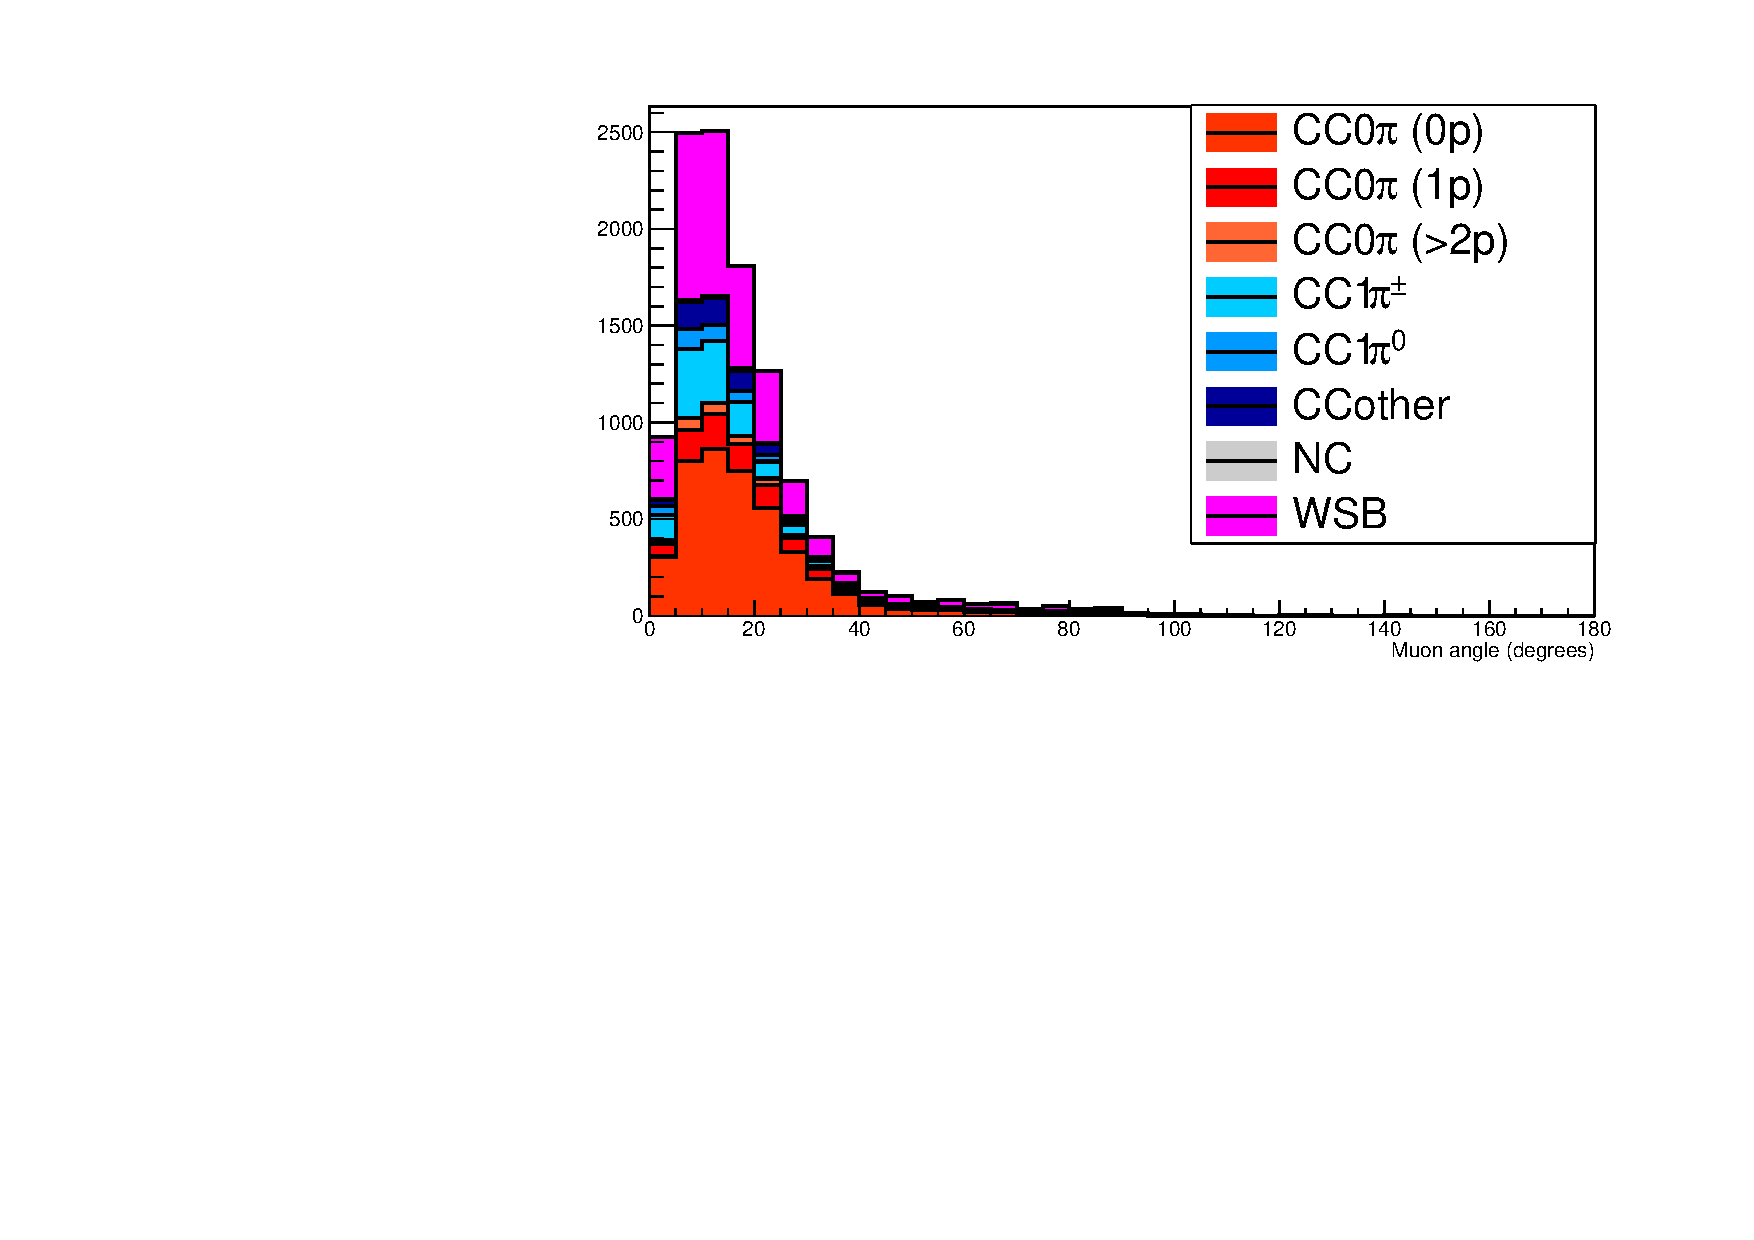
\includegraphics[width=0.55\linewidth, angle=270]{fig/RHCMuonAngle_StoppedOrThroughGoing.pdf}
%    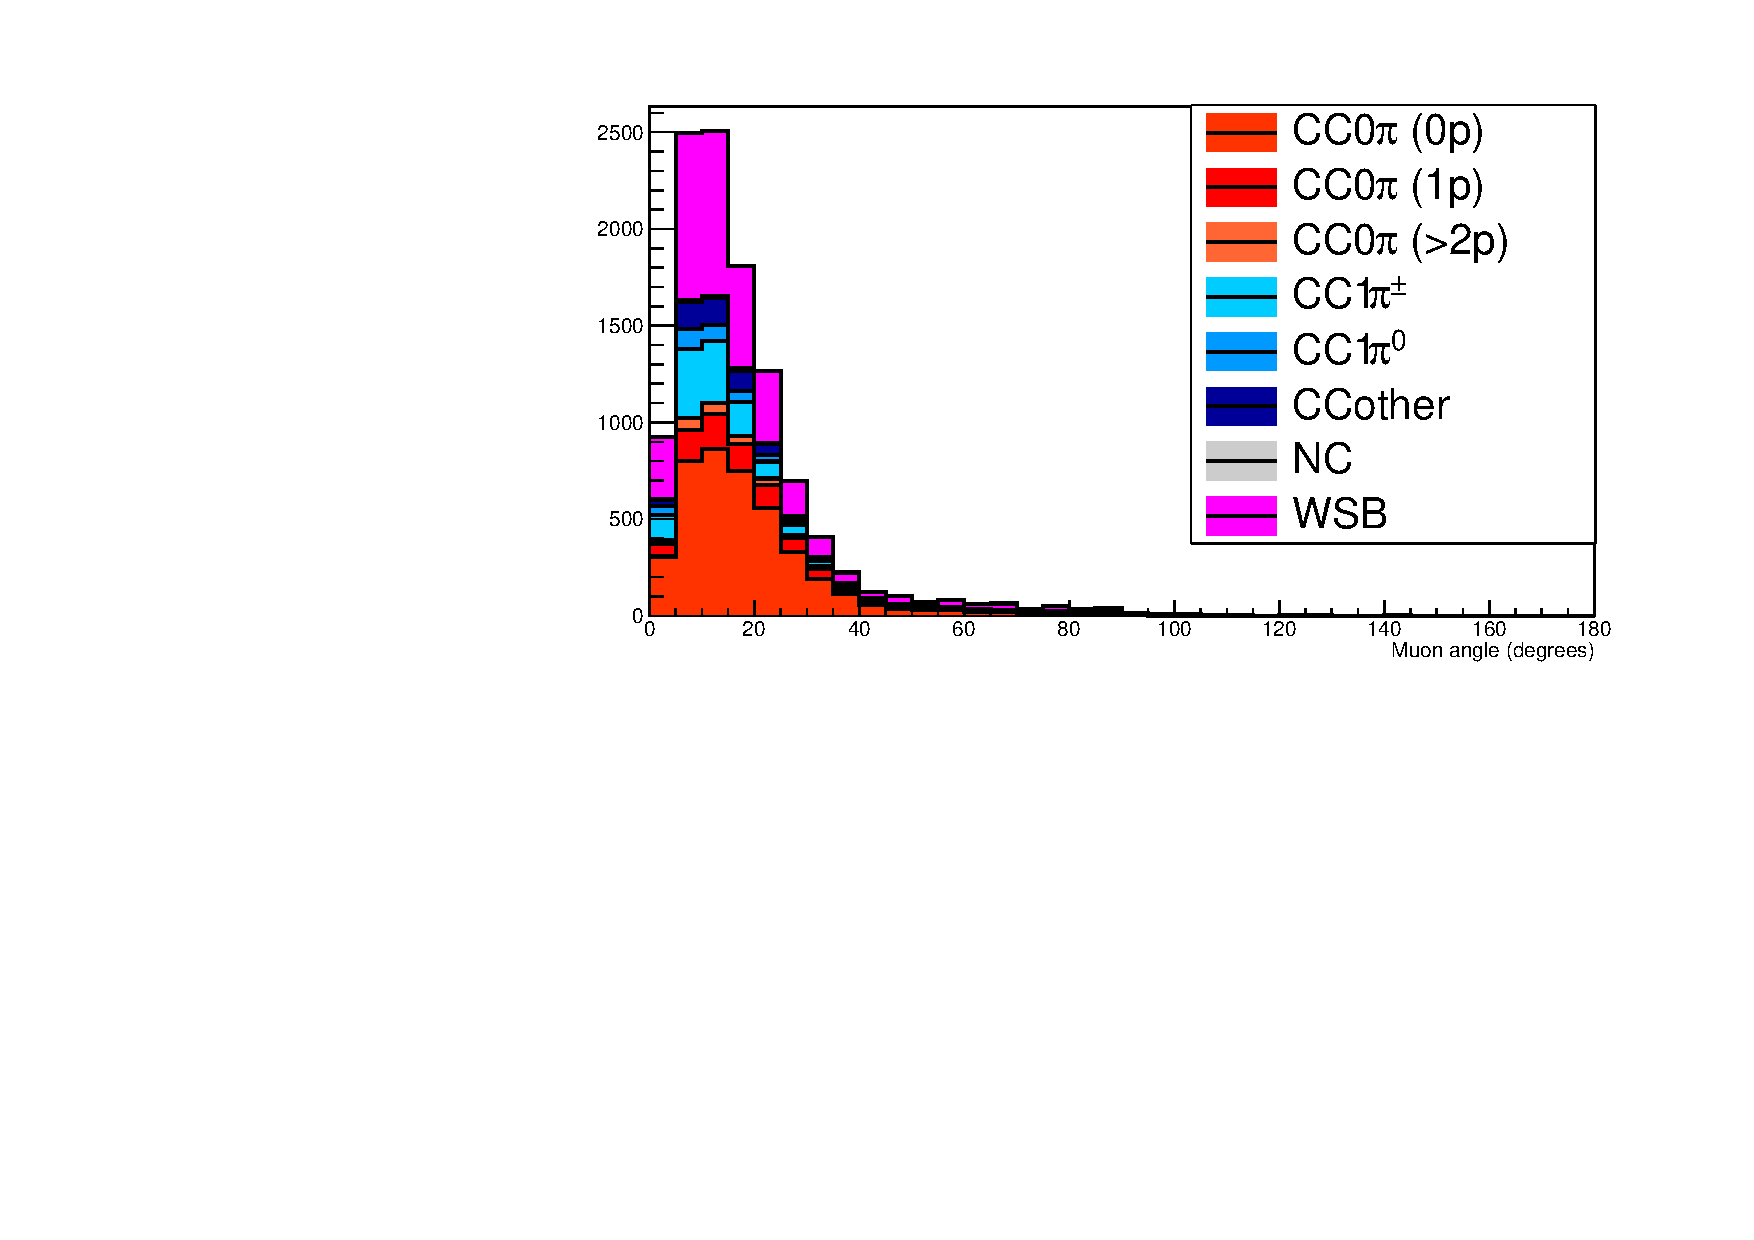
\includegraphics[width=\textwidth]{fig/RHCMuonAngle_StoppedOrThroughGoing.pdf}
    \end{subfigure}    
    \end{center}
  \caption{
The reconstructed angles of the longest tracks in the selected events in the neutrino-mode (left) and the antineutrino-mode (right).
}
\label{fig:angle_allcut}
\end{figure}
%
\begin{figure}[tbh]
 \begin{center}
  \begin{subfigure}{0.48\textwidth}
%     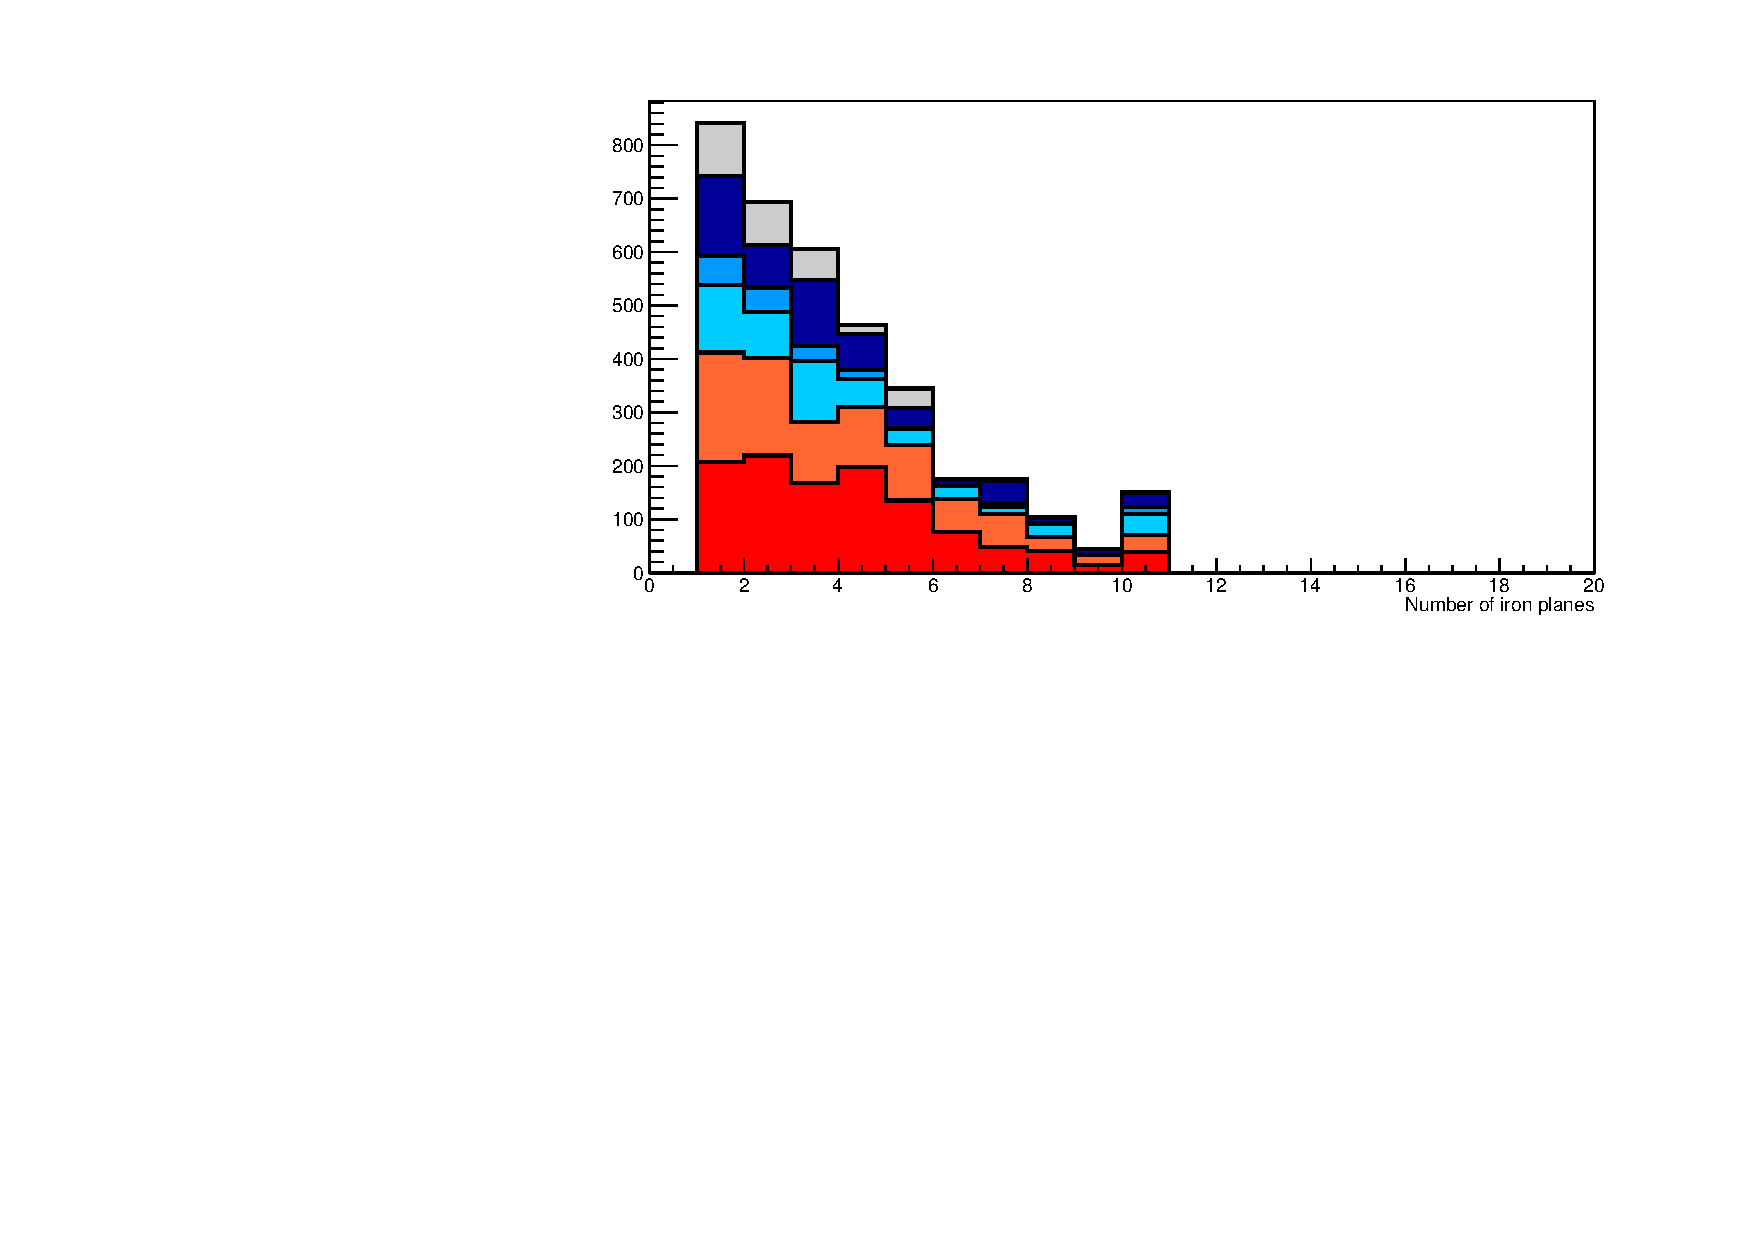
\includegraphics[width=\linewidth]{fig/FHCMuonPenetration_SideMRD_StoppedOrThroughGoing.pdf}
     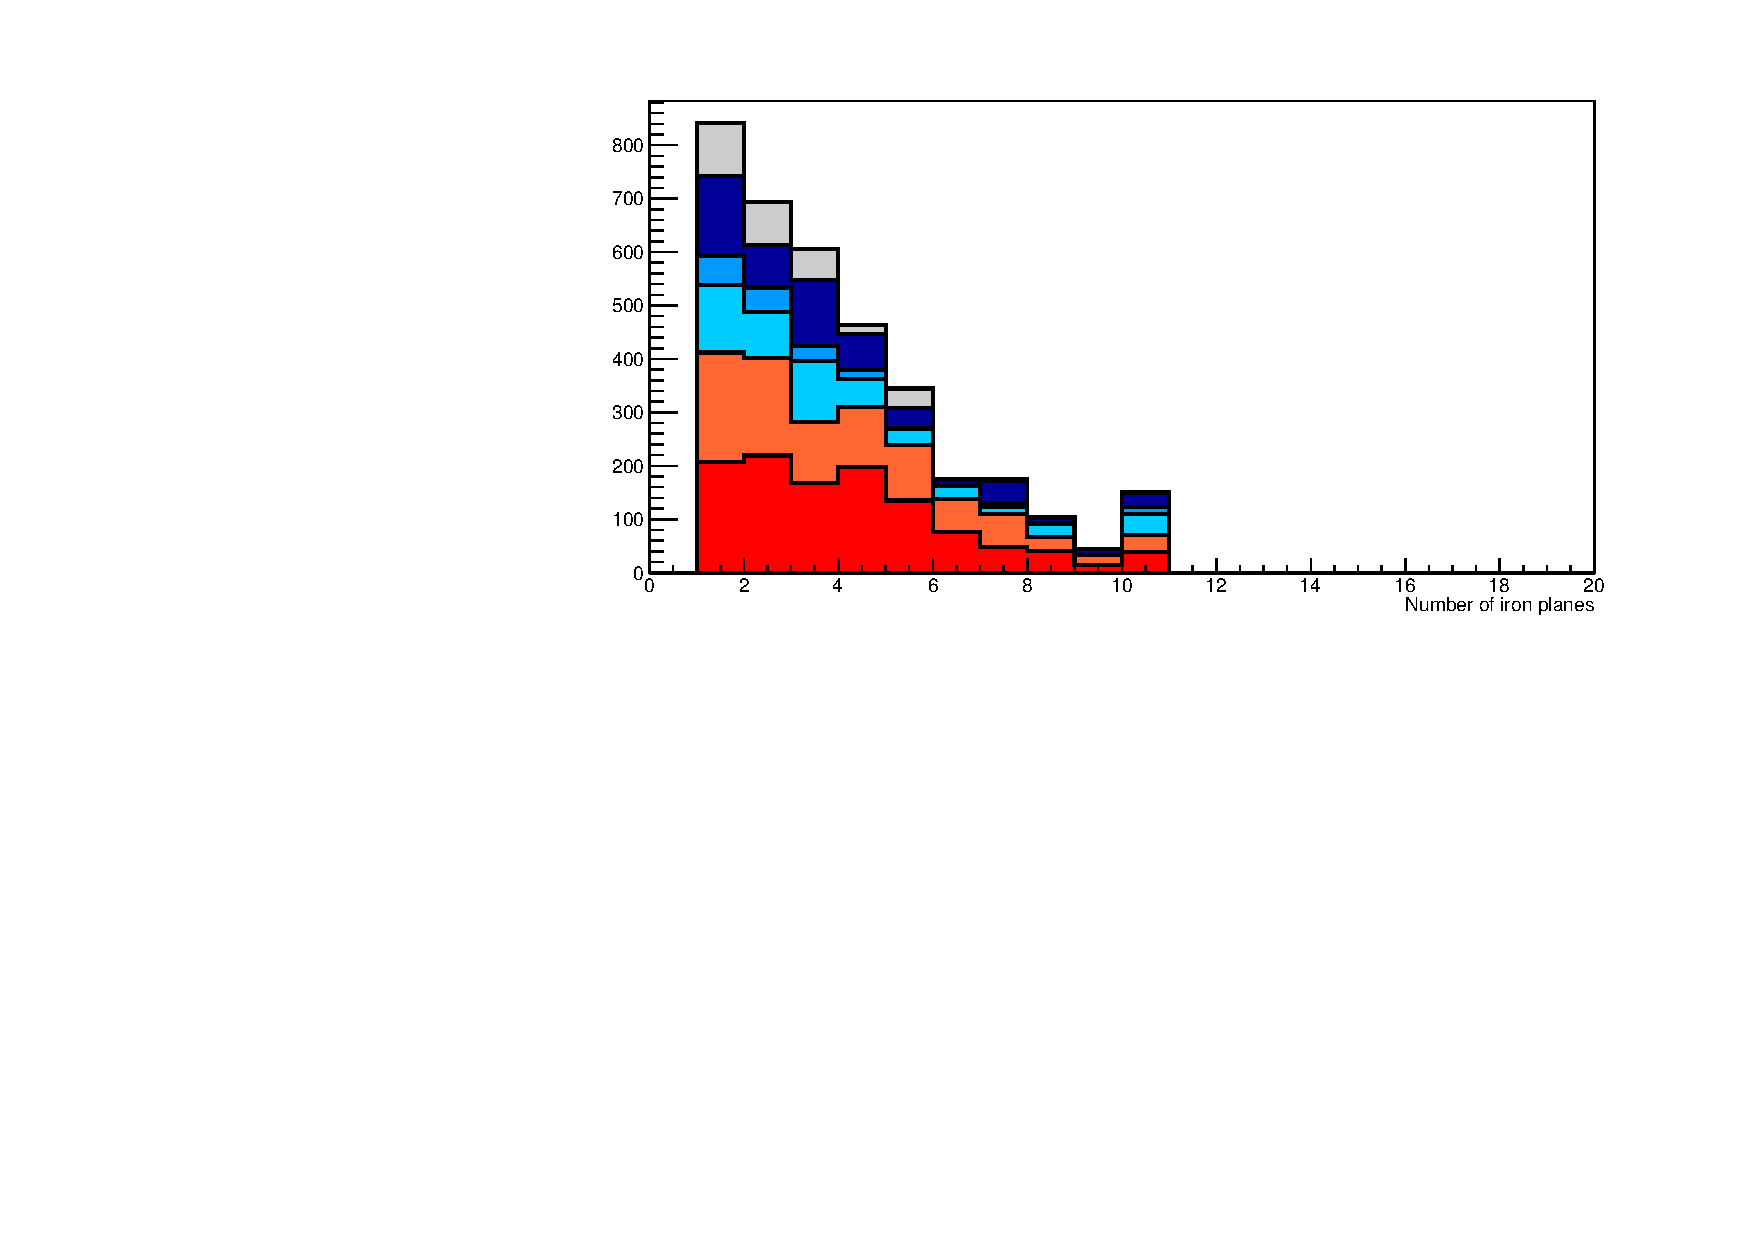
\includegraphics[width=0.55\linewidth, angle=270]{fig/FHCMuonPenetration_SideMRD_StoppedOrThroughGoing.pdf}
    \end{subfigure}
  \begin{subfigure}{0.48\textwidth}
%    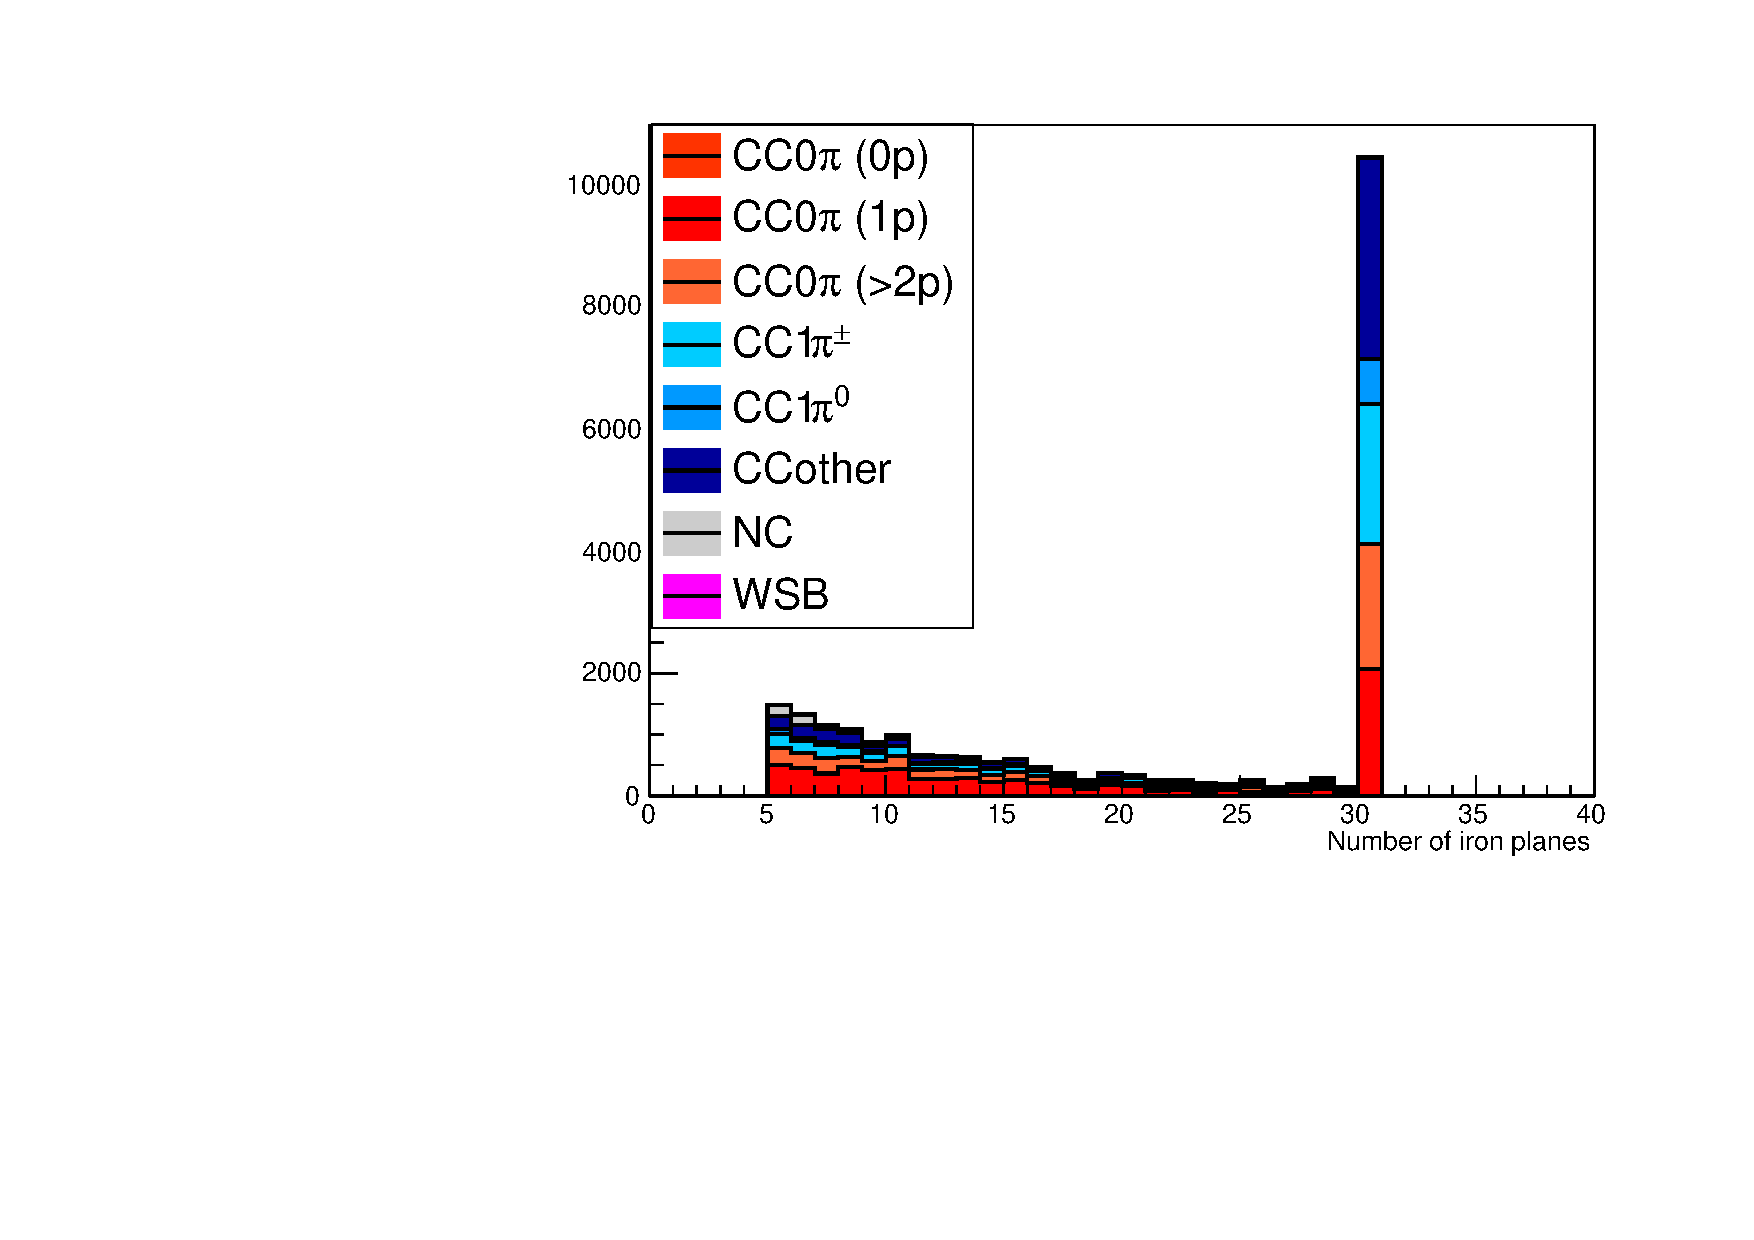
\includegraphics[width=\linewidth]{fig/FHCMuonPenetration_DownstreamMRD_StoppedOrThroughGoing.pdf}
    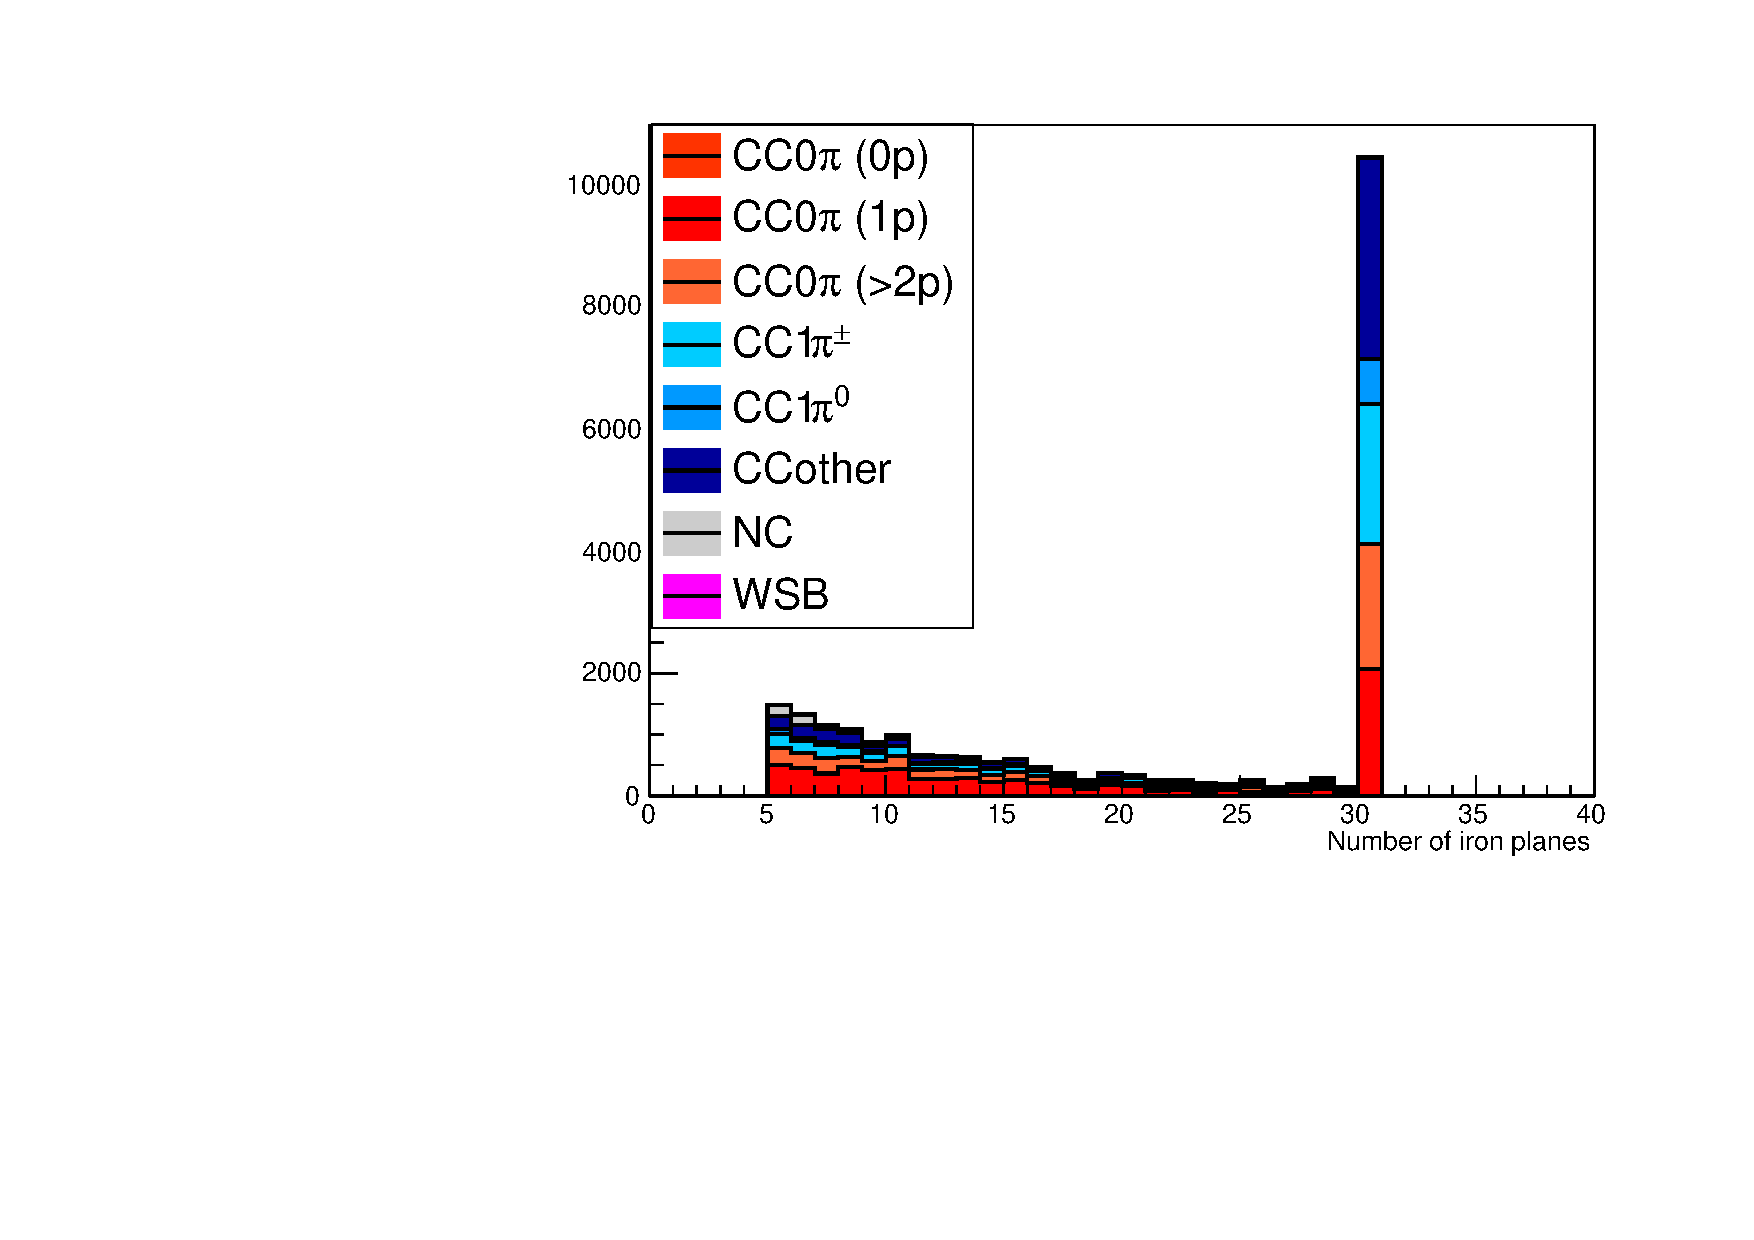
\includegraphics[width=0.55\linewidth, angle=270]{fig/FHCMuonPenetration_DownstreamMRD_StoppedOrThroughGoing.pdf}
    \end{subfigure}  
     \begin{subfigure}{0.48\textwidth}
%     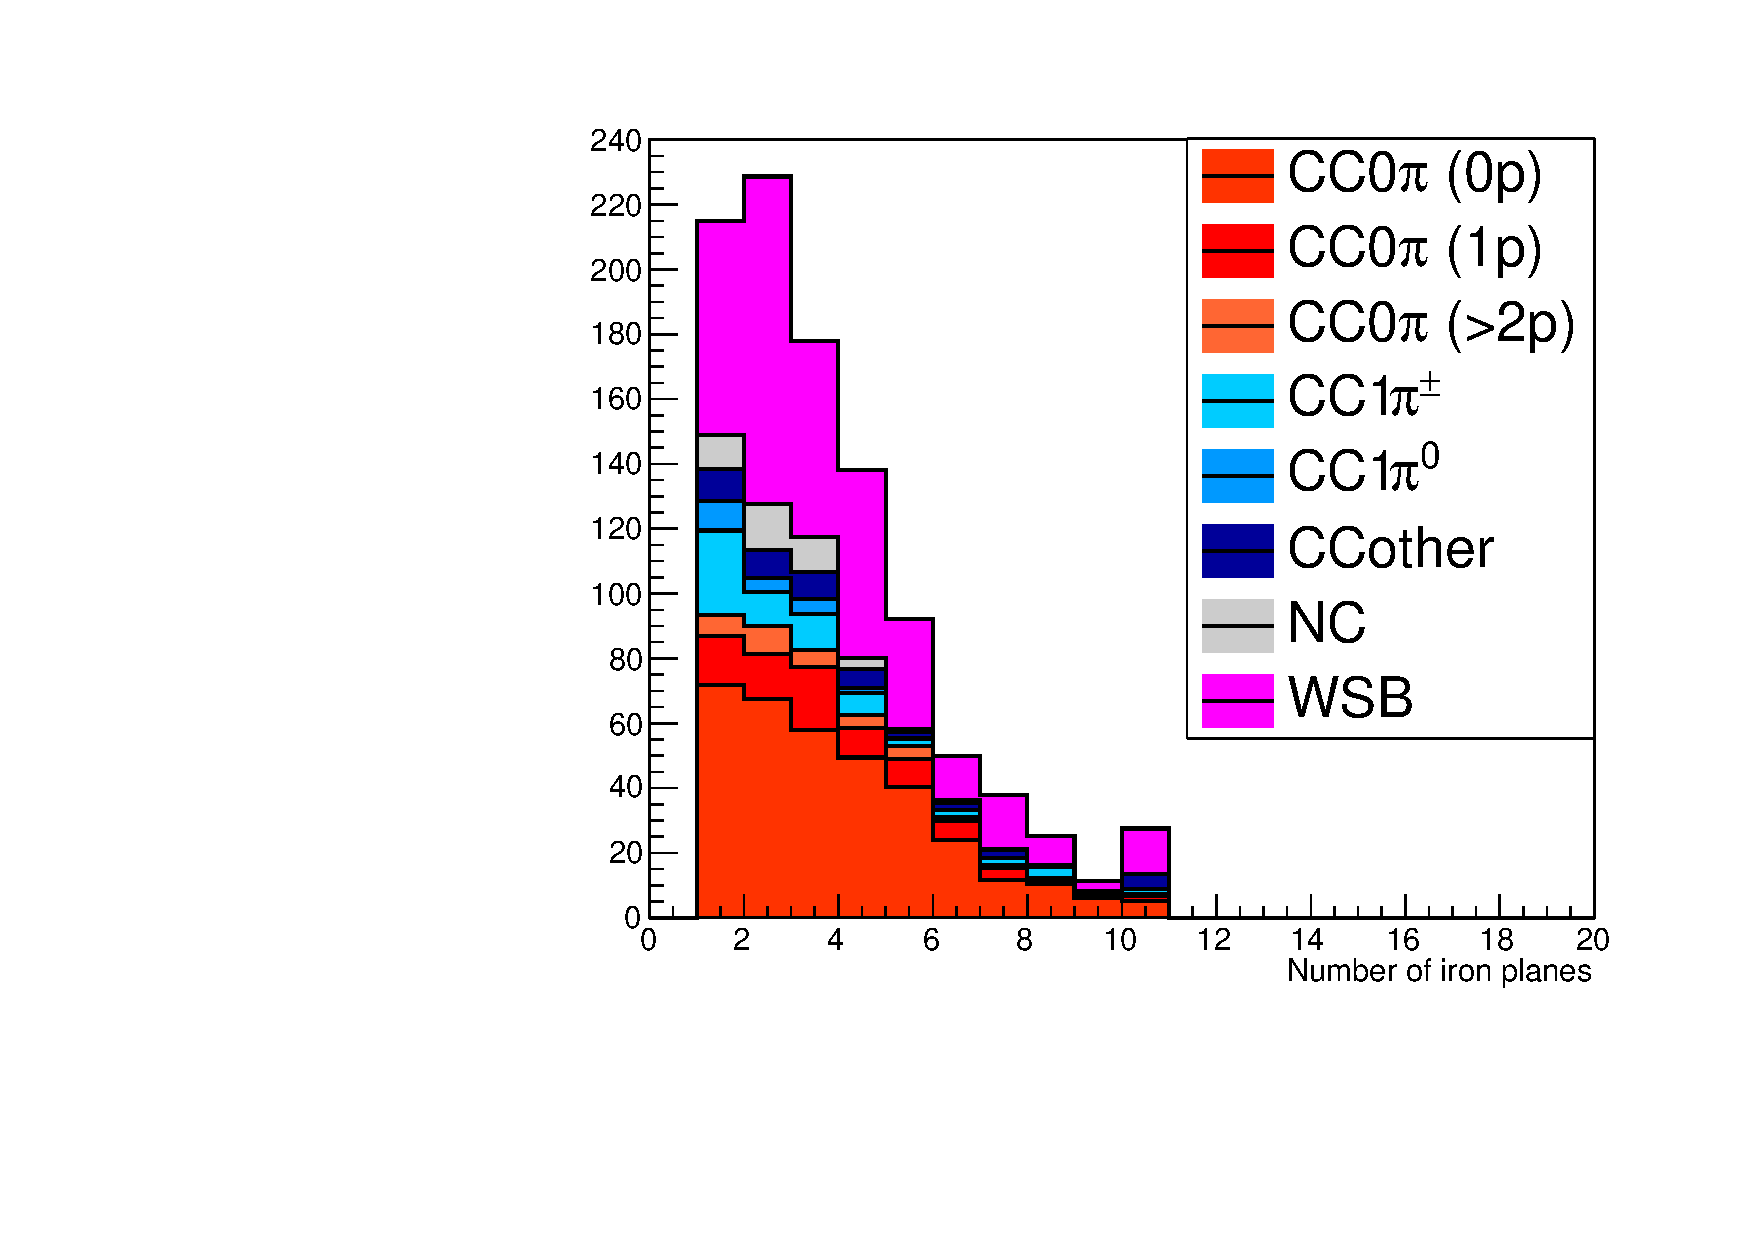
\includegraphics[width=\linewidth]{fig/RHCMuonPenetration_SideMRD_StoppedOrThroughGoing.pdf}
     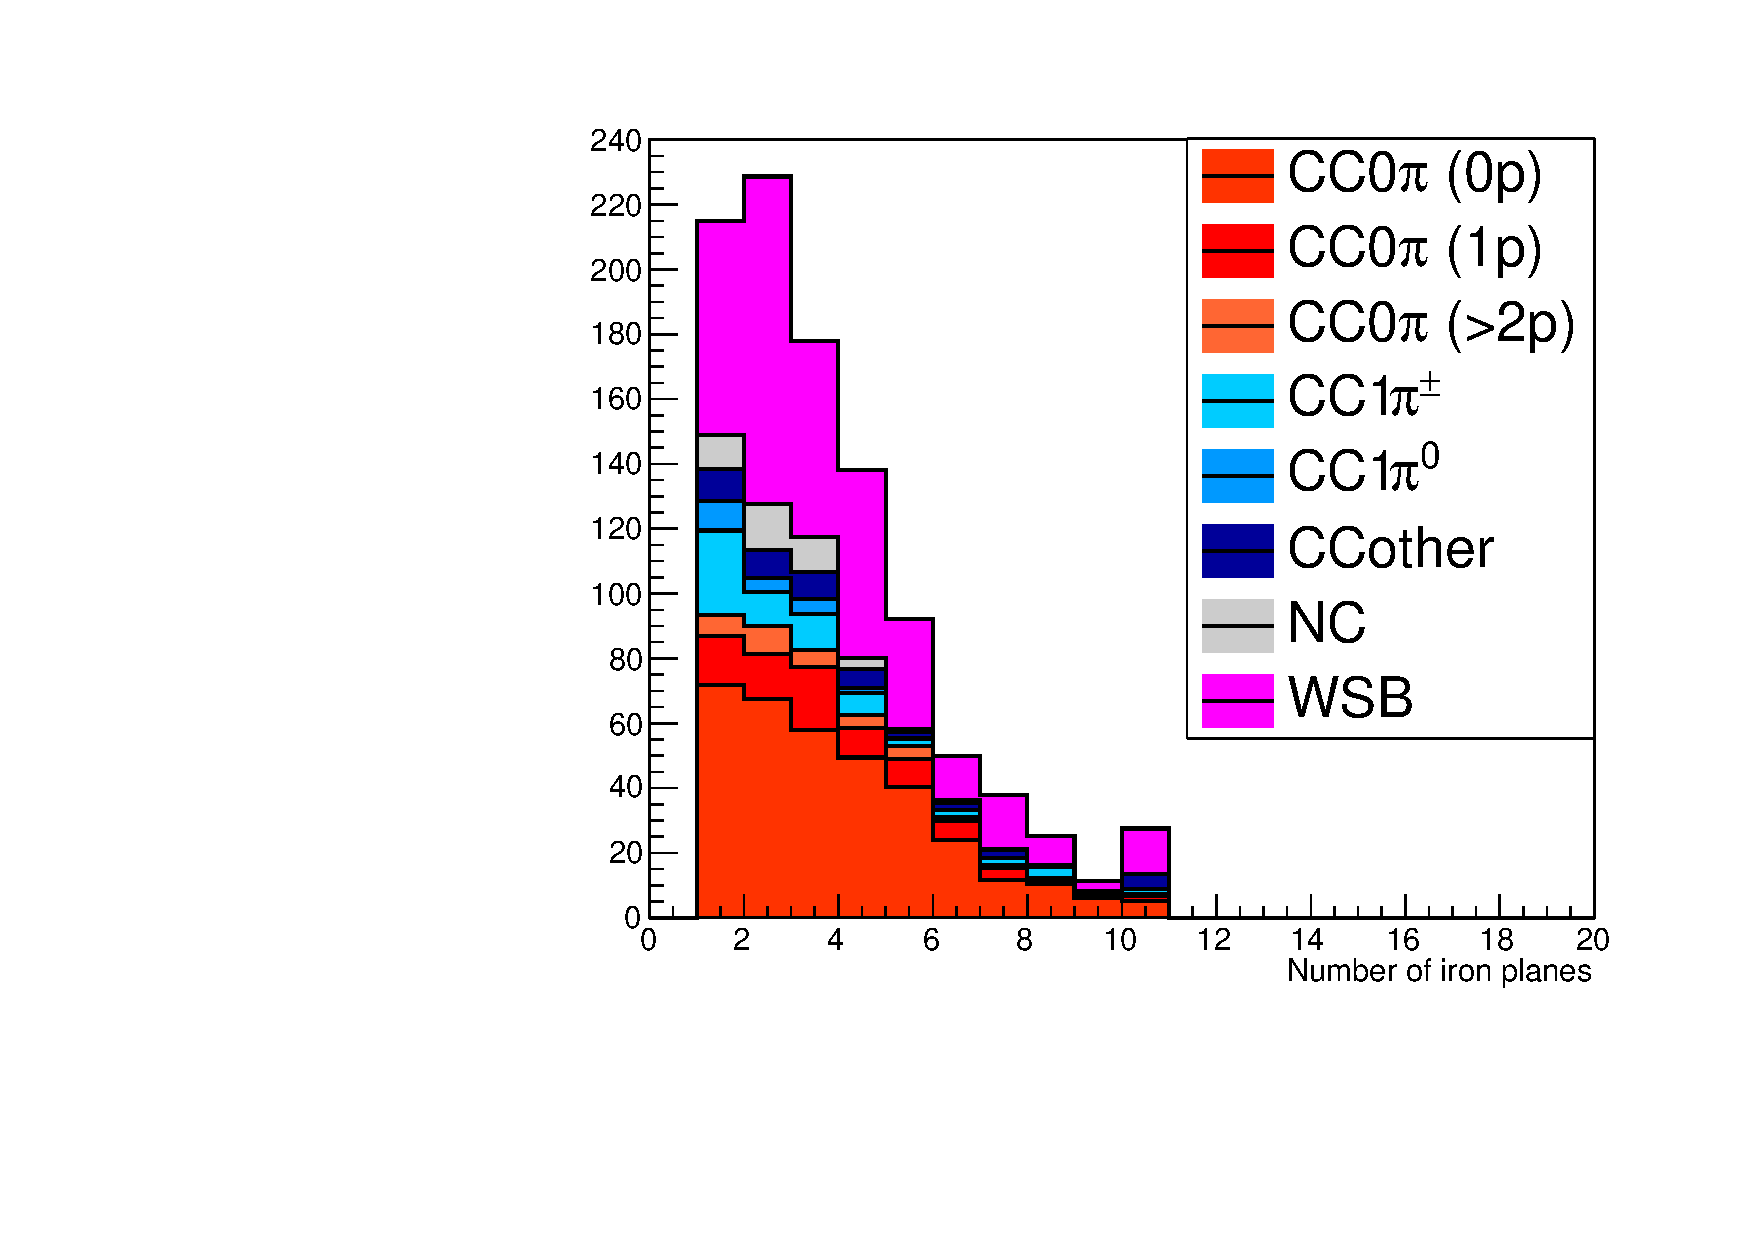
\includegraphics[width=0.55\linewidth, angle=270]{fig/RHCMuonPenetration_SideMRD_StoppedOrThroughGoing.pdf}
    \end{subfigure}
  \begin{subfigure}{0.48\textwidth}
%    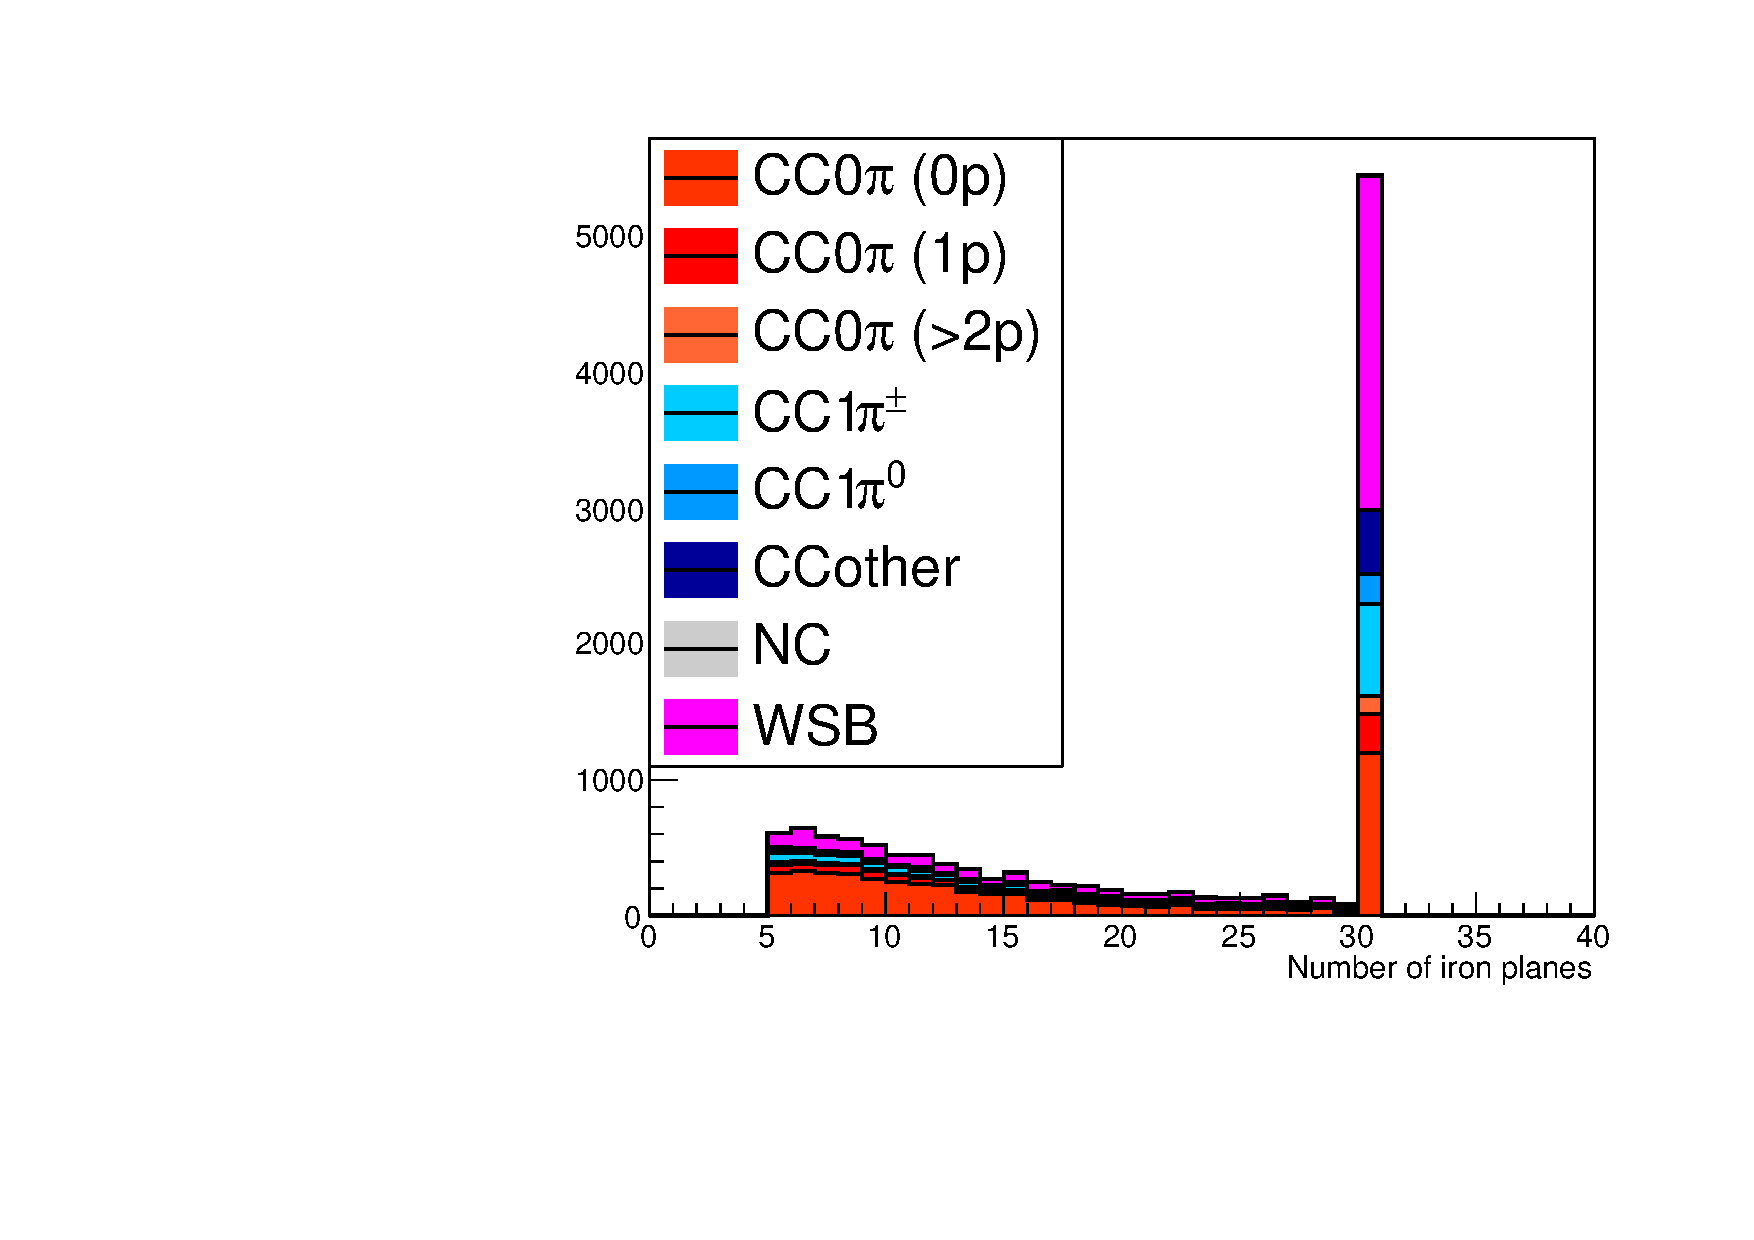
\includegraphics[width=\linewidth]{fig/RHCMuonPenetration_DownstreamMRD_StoppedOrThroughGoing.pdf}
    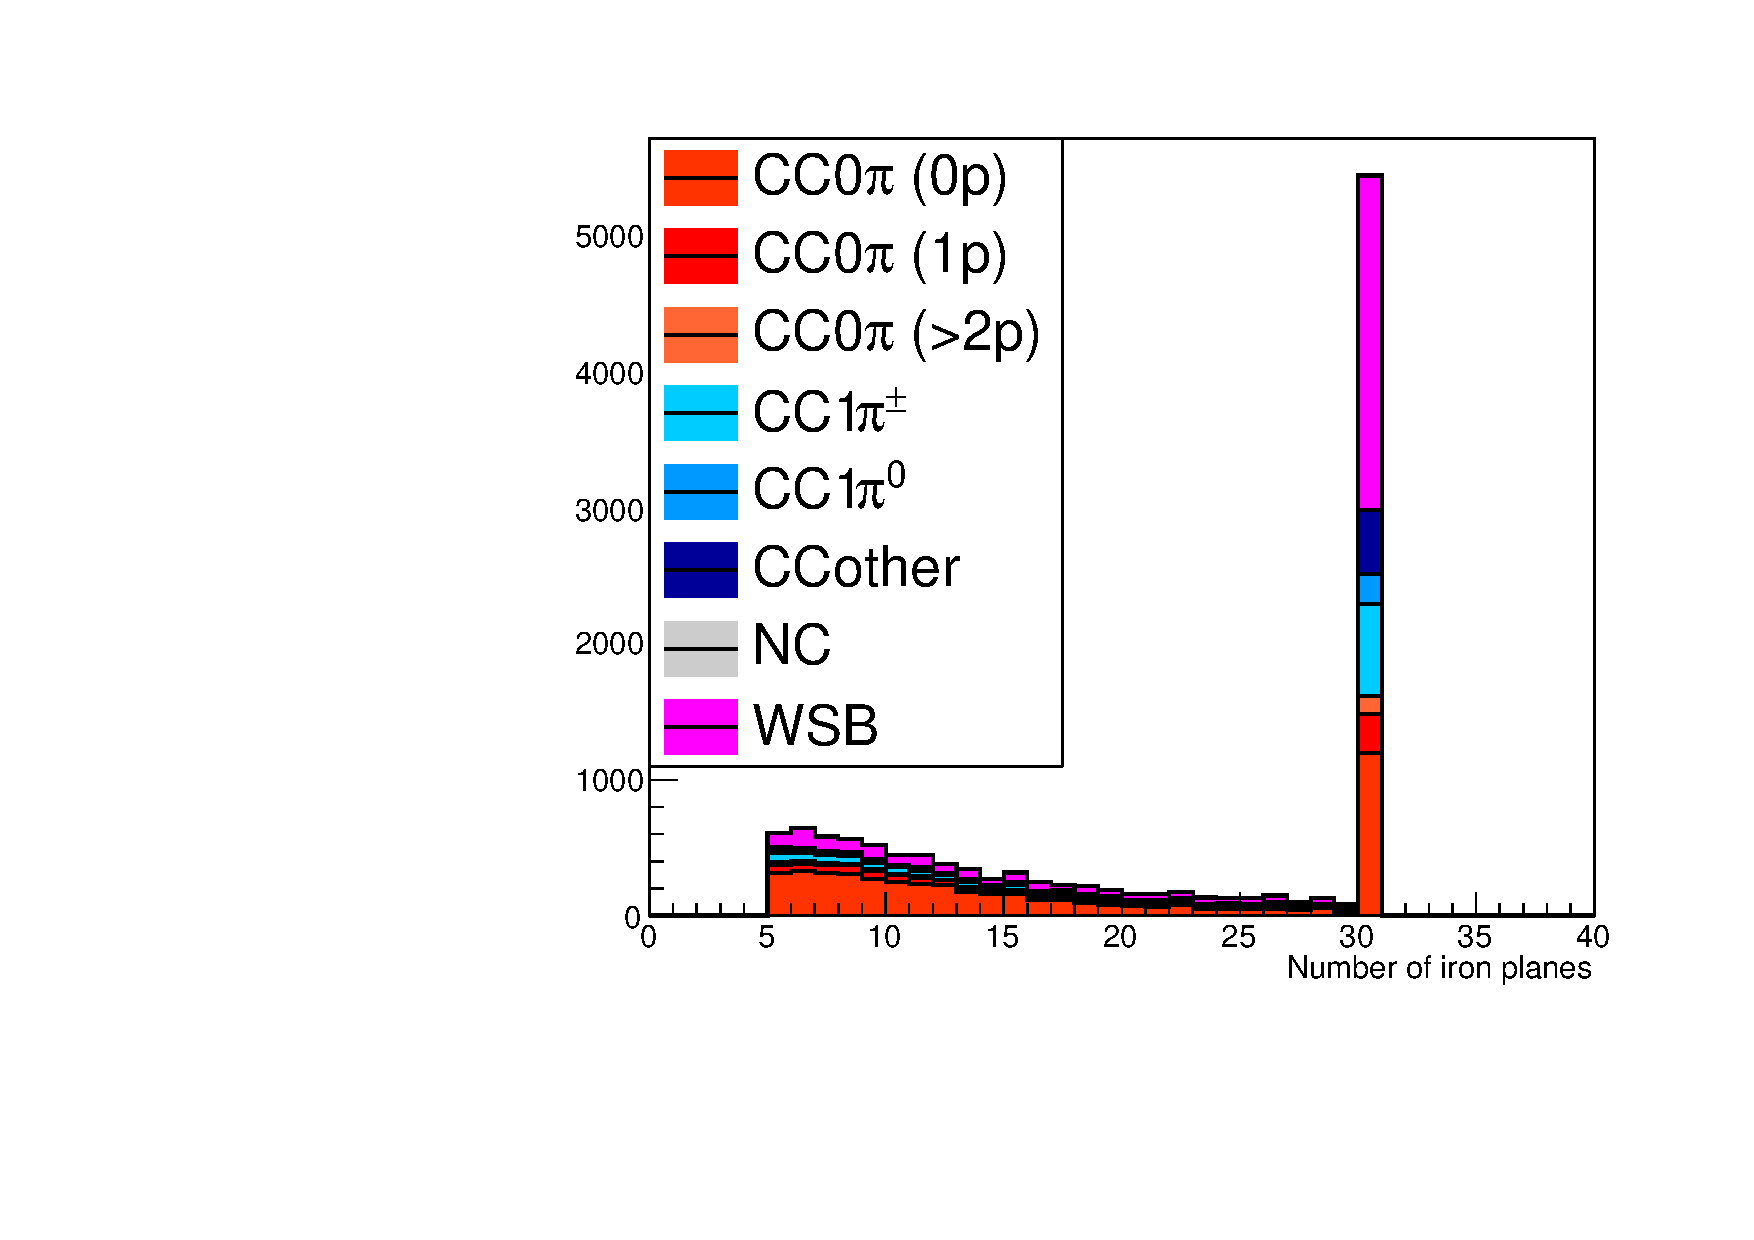
\includegraphics[width=0.55\linewidth, angle=270]{fig/RHCMuonPenetration_DownstreamMRD_StoppedOrThroughGoing.pdf}
    \end{subfigure}    
    \end{center}
  \caption{
Iron plane numbers in Side-MRD (left) and Baby-MIND (right) corresponding to the end points of the longest tracks in the selected events in the neutrino-mode (top) and the antineutrino-mode (bottom).
}
\label{fig:endpoint_longest_track}
\end{figure}



%Table \ref{tab:longest_track_particle} shows particles which produce the longest tracks in the selected events, and the fraction of muons is 85.6\%.
%
%\begin{table}[htb]
% \begin{center}
%   \caption{Particles which produce the longest tracks in the selected events.}
 %   \begin{tabular}{cc} \hline
 %     particles & fraction \\ \hline
 %     $\mu$ & 85.6\% \\
 %     $\pi^{+},\ \pi^{-}$ & 4.8\% \\
 %     p & 4.3\% \\
 %     e$^{+}$, e$^{-}$ & 4.5\% \\
 %     \hline
 %   \end{tabular}
 %   \label{tab:longest_track_particle}
 % \end{center}
% \end{table}

% Figure \ref{fig:eff_muon_angle_momentum_neutrino} shows detection efficiencies of muon tracks in the selected events as a function of muon's true angle and true momentum.
% The efficiency in the large angle region is low because Side-MRD modules only cover sides of the WAGASCI modules.
% The efficiency in the low momentum region is also low because more than two hits  are required to reconstruct the track in the WAGASCI detector.

% \begin{figure}[tbh]
%  \begin{center}
%   \begin{subfigure}{0.48\textwidth}
%     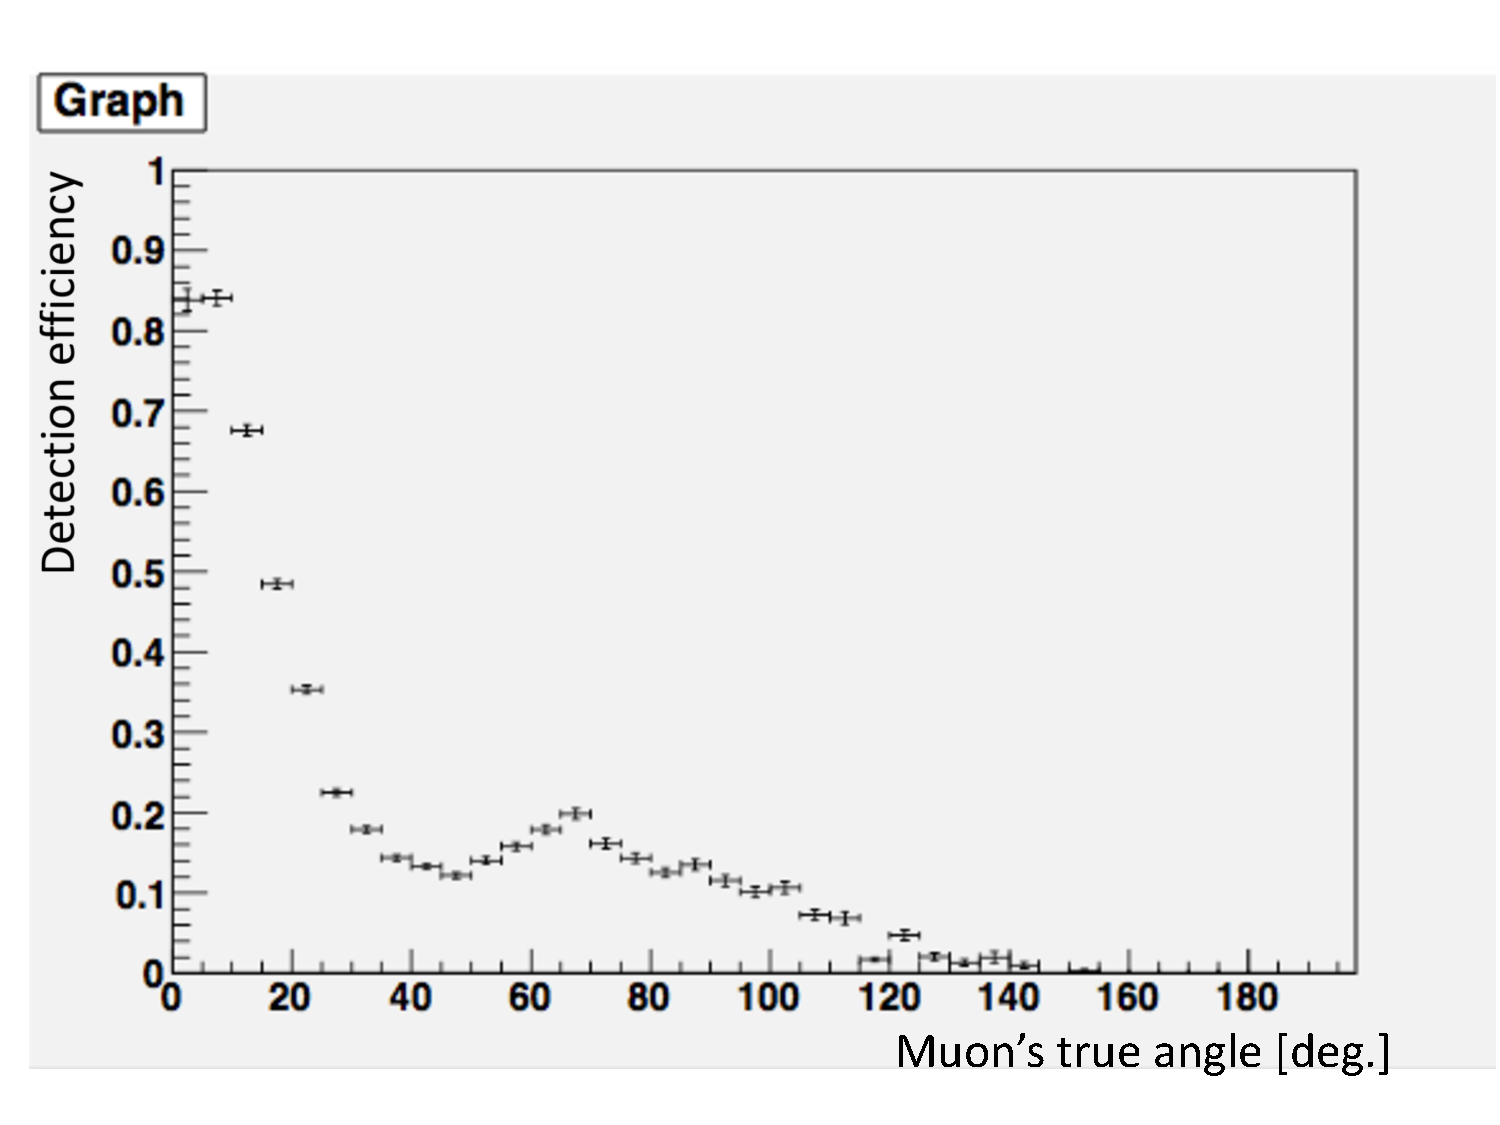
\includegraphics[width=\linewidth]{fig/eff_muon_angle_neutrino.pdf}
%    \end{subfigure}
%  \begin{subfigure}{0.48\textwidth}
%      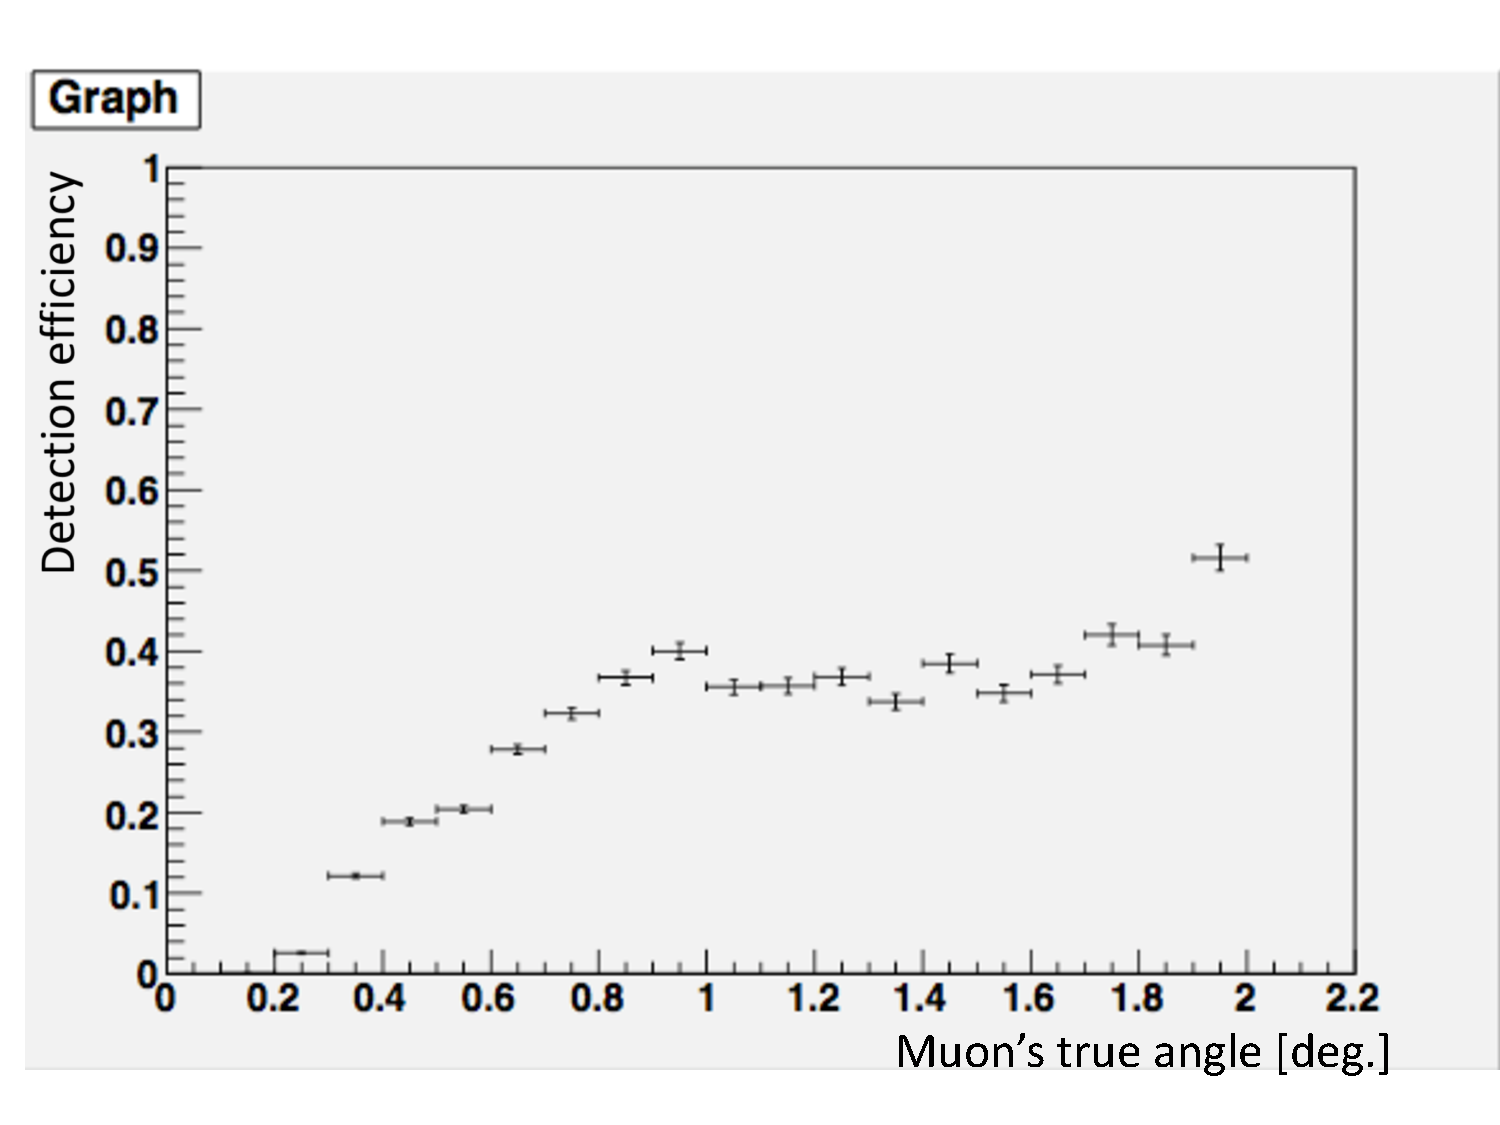
\includegraphics[width=\linewidth]{fig/eff_muon_momentum_neutrino.pdf}
%    \end{subfigure}    
%    \end{center}
%  \caption{
%Detection efficiencies of muon tracks in the selected events as a function of muon's true angle (left) and true momentum (right).
%}
%\label{fig:eff_muon_angle_momentum_neutrino}
%\end{figure}



\section{Group organization}

\section{Schedule}
We would like to start a physics data taking from T2K beam time after the summer shutdown in 2018.
By then, commissioning and tests of the detectors will be completed in J-PARC T59.
The experiment can run parasitically with T2K, therefore we request no dedicated beam time nor beam condition as discussed in the following section.

%Once the approved POT is accumulated, the WAGASCI modules will be removed from the experimental site, but we would like to keep the Baby-MIND and the Side-MRD modules on the B2 floor of the NM pit as common platforms of future neutrino experiments using the T2K neutrino beam.

\section{Requests}

\subsection{Neutrino beam}
The experiment can run parasitically with T2K, therefore we request no dedicated beam time nor beam condition.
As data taking periods, we request the `nominal' T2K one-year operation both for the neutrino beam and the antineutrino beam.
The T2K has been requesting $0.9\times10^{21}$~POT/year and actually accumulating about $0.7\times10^{21}$~POT/year in recent years.
For each year, starting from the Autumn,  T2K is running predominantly in the neutrino mode or in the antineutrino mode.
Our request is to have one-year neutrino-mode data and another one-year antineutrino mode data
assuming that the POT for the fast extraction in each year is more than $0.5\times10^{21}$~POT.

\subsection{Equipment request including power line}
We request the followings in terms of equipment on the B2 floor:
\begin{itemize}
\item {Site for the WAGASCI modules, Side-MRD modules and BabyMIND and their electronics system on the B2 floor of the near detector hall (Figure \ref{fig:all_detector_topview} and \ref{fig:location}).}
\item {Anchor points (holes) on the B2 floor to secure the WAGASCI modules, Side-MRD module and Baby-MIND, detailed floor plans to be communicated in a separate document.}
\item {Power line for the magnets in Baby-MIND: 400 V tri-phase 48-to-62 Hz, capable of delivering 12 kW. We have a wish for the magnet power line to be installed and available to us by beginning of March 2018.}
\item Electricity for electronics and water circulation system, 3 kW, standard Japanese electrical sockets.
	\begin{enumerate}
		\item Online PCs: 2.1 kW
		\item Electronics: 0.7 kW
		\item Water sensors: 1 kW
	\end{enumerate}
\item Air conditioner for cooling heat generation at Baby-MIND magnets, online PCs and electoronics
\item Beam timing signal and spill information
\item Network connection
\end{itemize}

The infrastructure for much of the above exists already.
Exceptions are the power line for the magnet and the electronics and holes in the B2 floor to anchor the detector support structures.

After this WAGASCI experiment, Baby MIND and Side-MRD's will remain if approved by J-PARC, and be used as common platforms of future neutrino experiments using the J-PARC neutrino beam.

\section{Conclusion}


\end{document}  